\documentclass{article}

% if you need to pass options to natbib, use, e.g.:
%     \PassOptionsToPackage{numbers, compress}{natbib}
% before loading neurips_2020

% ready for submission
% \usepackage{neurips_2020}

% to compile a preprint version, e.g., for submission to arXiv, add add the
% [preprint] option:
% \usepackage[nonatbib,final]{neurips_2020}
%\usepackage[nonatbib,preprint]{neurips_2020}

% to compile a camera-ready version, add the [final] option, e.g.:
%     \usepackage[final]{neurips_2020}

% to avoid loading the natbib package, add option nonatbib:
\usepackage[nonatbib]{neurips_2020}

\usepackage[utf8]{inputenc} % allow utf-8 input
\usepackage[T1]{fontenc}    % use 8-bit T1 fonts
% \usepackage[T2A]{fontenc}
\usepackage{hyperref}       % hyperlinks
\usepackage{url}            % simple URL typesetting
\usepackage{booktabs}       % professional-quality tables
\usepackage{amsfonts}       % blackboard math symbols
\usepackage{nicefrac}       % compact symbols for 1/2, etc.
\usepackage{microtype}      % microtypography

\usepackage{comment}
\usepackage{graphicx}
\usepackage{amsmath,amssymb} % define this before the line numbering.
\usepackage{color}
% \usepackage[width=122mm,left=12mm,paperwidth=146mm,height=193mm,top=12mm,paperheight=217mm]{geometry}
% \usepackage{cmap}					% поиск в PDF
\usepackage[english]{babel}	% локализация и переносы
% \usepackage[english,russian]{babel}
\usepackage{wrapfig}
\usepackage{longtable}

\usepackage{booktabs, multirow} % for borders and merged ranges
\usepackage{soul} % for underlines
\usepackage[table,dvipsnames]{xcolor} % for cell colors
\usepackage{changepage,threeparttable} % for wide tables

\usepackage[export]{adjustbox}
\usepackage{xfrac}
\usepackage{wrapfig}
\usepackage{placeins}
\usepackage{colortbl}
\definecolor{LightGray}{gray}{0.85}

% \usepackage[dvipsnames]{xcolor}
\newcommand{\lat}{\selectlanguage{english}}

% \iftoggle{nocomments}{
% 	\newcommand{\DZ}[1]{\ignorespaces}
% 	\newcommand{\EB}[1]{\ignorespaces}
% 	\newcommand{\OV}[1]{\ignorespaces}
% 	\newcommand{\LA}[1]{\ignorespaces}
% 	\newcommand{\VE}[1]{\ignorespaces}
% 	\newcommand{\DV}[1]{\ignorespaces}
% 	\newcommand{\todo}[1]{\ignorespaces}
% 	\newcommand{\todoshort}[1]{\ignorespaces}
% }{
% }

\newcommand{\MATTHIAS}[1]{\textcolor{Rhodamine}{\textbf{Matthias: #1}}}
\newcommand{\DZ}[1]{\textcolor{ForestGreen}{DZ: #1}}
\newcommand{\EB}[1]{\textcolor{magenta}{EB: #1}}
\newcommand{\AN}[1]{\textcolor{orange}{\textbf{AN: #1}}}
\newcommand{\LA}[1]{\textcolor{Plum}{\textbf{AA: #1}}}
\newcommand{\VI}[1]{\textcolor{blue}{\textbf{VI: #1}}}
\newcommand{\DV}[1]{\textcolor{Sepia}{\textbf{DV: #1}}}
\newcommand{\todo}[1]{\textcolor{red}{\textbf{TODO: #1}}}
\newcommand{\todoshort}[1]{\textcolor{red}{\textbf{#1}}}





\title{Scan2Part: Part Segmentation\\of~Real-World 3D~Scenes\\Supplementary Material}


% The \author macro works with any number of authors. There are two commands
% used to separate the names and addresses of multiple authors: \And and \AND.
%
% Using \And between authors leaves it to LaTeX to determine where to break the
% lines. Using \AND forces a line break at that point. So, if LaTeX puts 3 of 4
% authors names on the first line, and the last on the second line, try using
% \AND instead of \And before the third author name.

% \author{
%     Alexandr Notchenko , Vladislav Ishimtsev , Evgeny Burnaev\\
%   \texttt{\{a.notchenko,v.ishimtsev,e.burnaev\}@skoltech.ru} \\
% Skolkovo Institute of Science and Technology \\
% }
% \author{%
%   David S.~Hippocampus\thanks{Use footnote for providing further information
%     about author (webpage, alternative address)---\emph{not} for acknowledging
%     funding agencies.} \\
%   Department of Computer Science\\
%   Cranberry-Lemon University\\
%   Pittsburgh, PA 15213 \\
%   \texttt{hippo@cs.cranberry-lemon.edu} \\
  % examples of more authors
  % \And
  % Coauthor \\
  % Affiliation \\
  % Address \\
  % \texttt{email} \\
  % \AND
  % Coauthor \\
  % Affiliation \\
  % Address \\
  % \texttt{email} \\
  % \And
  % Coauthor \\
  % Affiliation \\
  % Address \\
  % \texttt{email} \\
  % \And
  % Coauthor \\
  % Affiliation \\
  % Address \\
  % \texttt{email} \\
% }

\begin{document}


\maketitle

This supplementary material contains the neccessary technical detail regarding the construction of our benchmark, methodological notes including the architecture of our network and loss functions, and extended experimental evaluation of our method.

\section{Scan2Part benchmark}
\label{supsec:scan2part-dataset-detail}



\paragraph{Aligning PartNet and ShapeNet databases}
\label{dataset:processing-detail}
% \LA{maybe compress this, renaming to "Aligning PartNet and ShapeNet databases"}
PartNet~\cite{mo2019partnet} is a hierarchical instance-level parts dataset of labels for the subset of the ShapeNet~\cite{chang2015shapenet} database.
Specifically, PartNet provides part-level annotation for the geometry of objects in the ShapeNet.
However, due to its annotation procedure, PartNet does not preserve the original coordinate system for respective ShapeNet objects, thus, objects in PartNet differ from those in ShapeNet by a rigid transformation; we thus set out to restore the original coordinate system.
To find the rotation matrix between coordinate systems, we use the following alignment process for each object:
\begin{enumerate}
    \item We sample 20 different rotation angles corresponding to the vertices of the convex regular dodecahedron.
    Each rotation angle corresponds as the initial alignment matrix of the object from ShapeNet for alignment to corresponding location in PartNet.
    \item We perform Point-to-point ICP alignment~\cite{besl1992method} separately for each initial alignment matrix.
    \item We select the best one out of 20 alignment results where the Euclidean distance between the original ShapeNet shape and the rotated PartNet shape is minimal.
\end{enumerate}



\paragraph{Statistics on the available alignments. }
\label{dataset:alignments-statistics}
Our Scan2Part dataset leverages 9\,DoF alignments provided by Scan2CAD benchmark~\cite{avetisyan2019scan2cad} and parts labeling from PartNet~\cite{mo2019partnet}, both focusing on different (but significantly intersecting) subsets of ShapeNet.
Thus, we restrict our consideration to shapes where 9\,DoF poses exist simultaneously with part-level annotations.
Table~\ref{tab:object_presence} displays aggregated statistics on the availability of part-level annotation for shapes with known alignments, with Table~\ref{tab:class_presence} detailing this statistics across major classes.

% But Scan2CAD also works with very limited subset of ShapeNet. The intersection over these subsets is around 2477 ShapeNet models that are presented in both datasets. Exact numbers can be taken from CAD-Deform supplementary --- I copied these tables to  and~\ref{tab:class_presence}

\begin{table}[!h]
\caption{Overall statistics on the numbers of categories, instances, and correspondences present in our datasets.}
\centering
\resizebox{0.7\textwidth}{!}{%
\begin{tabular}{l ccc}
\toprule
\textbf{Collection} & \textbf{Categories} & \textbf{Instances} & \textbf{Corresp.} \\
\midrule
Scan2CAD~\cite{avetisyan2019scan2cad} & 35 & 3,049 & 14,225 \\
           \qquad w/parts annotations & 24 & 2,477 & 12,246 \\
\bottomrule
\end{tabular}
}
\label{tab:object_presence}
\end{table}

\begin{table}[ht!]
\caption{The top~15~most frequent ShapeNet categories in Scan2CAD dataset including a detailed information on those with the availability of the corresponding parts annotations. The symbol $\downarrow$ indicates the sorting order.}
\centering
\resizebox{0.6\textwidth}{!}{%
\begin{tabular}{l cc cc}
\toprule
    \multirow{2}{*}{\textbf{Name}}
    & \multicolumn{2}{c}{\textbf{Scan2CAD}}
    & \multicolumn{2}{c}{\textbf{PartNet $\cap$ Scan2CAD}}  \\
    & corresp.
    & shapes
    & corresp. $\downarrow$ 
    & shapes \\
\midrule
% \multicolumn{5}{l}{\textit{Shape categories used in our evaluation:}} \\
chair & 4677 & 652 & 4351 & 632 \\
table & 2616 & 830 & 2594 & 822 \\
cabinet & 1401 & 310 & 1258 & 294 \\
trash bin & 1044 & 89 & 1042 & 88 \\
bookshelf & 824 & 150 & 812 & 145 \\
display & 770 & 165 & 762 & 161 \\
% \midrule
% \multicolumn{5}{l}{\textit{Shape categories NOT used in our evaluation:}} \\
bed & 355 & 50 & 342 & 47 \\
file cabinet & 294 & 70 & 290 & 68 \\
bag & 165 & 9 & 165 & 9 \\
lamp & 135 & 55 & 135 & 55 \\
bathtub & 474 & 96 & 129 & 25 \\
microwave & 99 & 37 & 98 & 36 \\
sofa & 577 & 247 & 60 & 20 \\
laptop & 51 & 24 & 51 & 24 \\
keyboard & 62 & 11 & 48 & 9 \\
flowerpot & 38 & 12 & 37 & 11 \\
dishwasher & 37 & 14 & 29 & 12 \\
clock & 15 & 6 & 15 & 6 \\
bowl & 12 & 3 & 12 & 3 \\
faucet & 22 & 7 & 7 & 4 \\
basket & 85 & 32 & 6 & 3 \\
bottle & 3 & 2 & 1 & 1 \\
jar & 1 & 1 & 1 & 1 \\
cap & 1 & 1 & 1 & 1 \\
\midrule
\textbf{Total} & 14,225 & 3,049 & 12,246 & 2,477 \\
\bottomrule
\end{tabular}
}
\label{tab:class_presence}
\end{table}



\paragraph{Taxonomy processing details. }
\label{dataset:taxonomy-detail}
% 1. description of the taxonomy
The original PartNet taxonomy is represented by a set of classes $\mathbb{P} = \{\text{chair}, \text{chair base}, \text{chair base footrest ring}, \ldots, \text{sofa}, \ldots\}$ arranged in a hierarchy $\mathbb{P}_1, \mathbb{P}_2, \ldots$ such that each level $\mathbb{P}_k$ at depth $d_k$ from the root in the hierarchy contains a subset of classes from $\mathbb{P}$: $\mathbb{P}_k \subset \mathbb{P}$. 
In this paper, we start with the existing taxonomy represented by structural relations between the sets $\mathbb{P}, \mathbb{P}_1, \mathbb{P}_2, \ldots$ and adapt it to real-world 3D scans, constructing a modified taxonomy with a set of classes $\mathbb{C} = \mathbb{C}_1 \cup \mathbb{C}_2 \cup \ldots$. 
Specifically, we perform the following series of steps: 
\begin{enumerate}
    \item Trivially, we only select classes in $\mathbb{P}$ corresponding to part categories of 3D shapes available in Scan2CAD, see Tables~\ref{tab:object_presence}--\ref{tab:class_presence}.

    % 2. compressing taxonomy by merging classes
    \item To detail the algorithm outlined in the main text, we construct a per-voxel annotation by first selecting triangles of aligned meshes spatially located in each voxel and next assigning part categories of the selected triangles $P_1 \in \mathbb{P}_1, P_2 \in \mathbb{P}_2, \ldots$ with the highest numbers of representatives at each granularity level to voxels. 
    This results in certain part categories, particularly fine-grained ones (e.g., keyboard buttons), being under-represented in the dataset.
    Table~\ref{tab:taxonomy_structure_by_threshold} summarizes statistics of part categories with numbers of representatives exceeding a series of thresholds.
    We select a value of the threshold at 1800\,voxels, aiming to strike a good balance between dataset diversity and occurrence of individual categories, and omit the significantly under-represented classes from our taxonomy.

    % 3. compressing taxonomy by pruning the taxonomy tree
    \item We prune the resulting taxonomy tree by collapsing branches where only a single child node exists, keeping part categories in leaves. 

\end{enumerate}

As an application, we construct a hierarchical annotation of 3D reconstructed scenes from ScanNet~\cite{dai2017scannet} at three granularity levels $\mathbb{C}_1, \mathbb{C}_2, \mathbb{C}_3$. Figure~\ref{fig:more_teasers} displays more instances of 3D shapes in our Scan2Part benchmark, and Figure~\ref{fig:part_level_variation_voxels} focuses on example instances colored according to different granularity levels in the taxonomy.

% compressing taxonomy by merging classes. Actually, Partnet taxonomy already have merged classes in the way that we merge them: all tables legs comes from the same class. Here we just can highlight that we have a DoF for choosing level of merging and argue the chosen level. I created picture\ref{fig:three_tables} for varying the level of merging



% 3. compressing taxonomy by pruning the taxonomy tree

%  • [126] We further describe the main steps taken to create our Scan2Part benchmark below, leaving the detailed discussion of the technicalities for the supplementary. Annotation schema for our dataset is shown in Figure 3. — здесь, насколько я понял, нужно подробно описать про разные уровни разметки, про разные уровни агрегации разметки. Также вероятно к этому куску относиться и treemop, который рисовал Саша


\begin{figure}[!t]
\label{fig:three_tables}
\centering
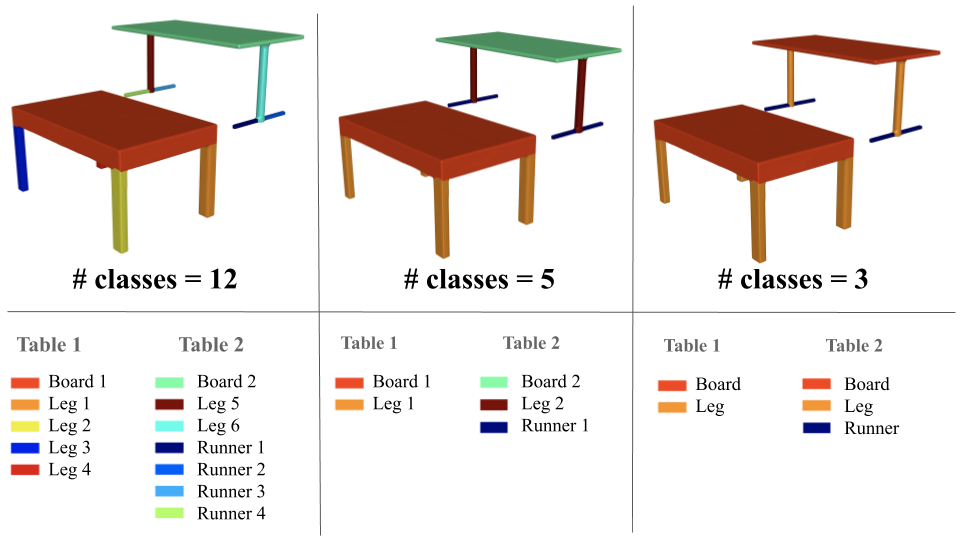
\includegraphics[width=0.9\textwidth]{images/three_tables}
\caption{Different rules for combining the part trees of all the objects. (left) if colors of all the legs are different, (center) if color of legs depends on the the table, (right) if color of all legs are the same. Instance information doesn't always provide relevant information about the part of the object, and is redundant in most samples.}
\end{figure}







\paragraph{Taxonomy statistics. }
\label{dataset:taxonomy-stats}
% say something about taxonomy 

% Under closer examination, we discovered that most of the parts do not have a unique shape making the task of instance segmentation for parts very hard to solve and not necessary for practical scene segmentation task. 



% Плюс учитывая то, что скидывал раньше Саша, supplementary должно состоять как минимум из следующего:
%  1. Детали датасета. Разные уровни разметки (есть), разные уровни агрегации (есть)
%  2. Детальное описание таксономии. Табличка “количество уровней в дереве” X “порог обрубания вершин”, в ячейках количество классов (есть), аргументация о выборе оптимального порога 1800 (нет), полная таксономия на трёх уровнях (есть).


Table~\ref{tab:taxonomy_structure_by_threshold} displays class statistics with taxobtained by thresholding at different values of the class occurrence. 

%  • [146] We proceed with this reduction by first choosing an appropriate occurrence threshold (we pick 1800 voxels, but demonstrate the effect of different threshold values in the supplementary) and remove classes that have smaller number of representatives in the dataset. — здесь необходимо привести табличку (количество уровней в дереве X порог обрубания вершин). Табличка посчитана, но непонятно, как из неё сделать вывод, что порог 1800 вокселей — оптимальный. @ чем ты руководствовался при выборе этого порога?

\begin{table}[!ht]
    \centering
    \caption{The effect of class occurrence threshold on taxonomy structure. For each depth $d_k$ in the PartNet taxonomy, we display the number of classes $|\mathbb{C}_k|$ with occurrence values greater than \#\,Voxels threshold (left column). The shaded row approximately corresponds to our taxonomy structure.}
    \begin{tabular}{r cccccccc}
        \toprule
        & \multicolumn{8}{c}{Depth $d_k$} \\
        \cmidrule{2-9}
        \#\,Voxels & 1 & 2 & 3 & 4 & 5 & 6 & 7 & 8 \\
         & (object) & (coarse) & & & & & & (fine) \\
        \midrule
        0    & 18 & 50 & 133 & 223 & 269 & 302 & 306 & 307 \\
        1K   & 15 & 42 &  86 & 119 & 142 & 147 & 152 & 156 \\
        \rowcolor{LightGray}
        2K   & 12 & 28 &  60 &  96 & 117 & 122 & 127 & 131 \\
        5K   & 11 & 21 &  43 &  70 &  86 &  89 &  93 &  97 \\
        10K  & 11 & 19 &  35 &  57 &  70 &  72 &  74 &  75 \\
        20K  &  8 & 15 &  26 &  43 &  50 &  51 &  52 &  52 \\
        50K  &  6 & 13 &  19 &  27 &  29 &  29 &  29 &  29 \\
        100K &  6 & 11 &  15 &  21 &  22 &  22 &  22 &  22 \\
        \bottomrule
    \end{tabular}
    \label{tab:taxonomy_structure_by_threshold}
\end{table}


% \VI{DONE: more figures displaying taxonomies for example objects (like Figure 1 in main text)}
%  5. Несколько дополнительных примеров пропажи лейблов в результате перехода PartNet -> Scannet (нет) (наподобие рисунка 1 основной статьи)

\begin{figure}[!t]
\label{fig:more_teasers}
\centering
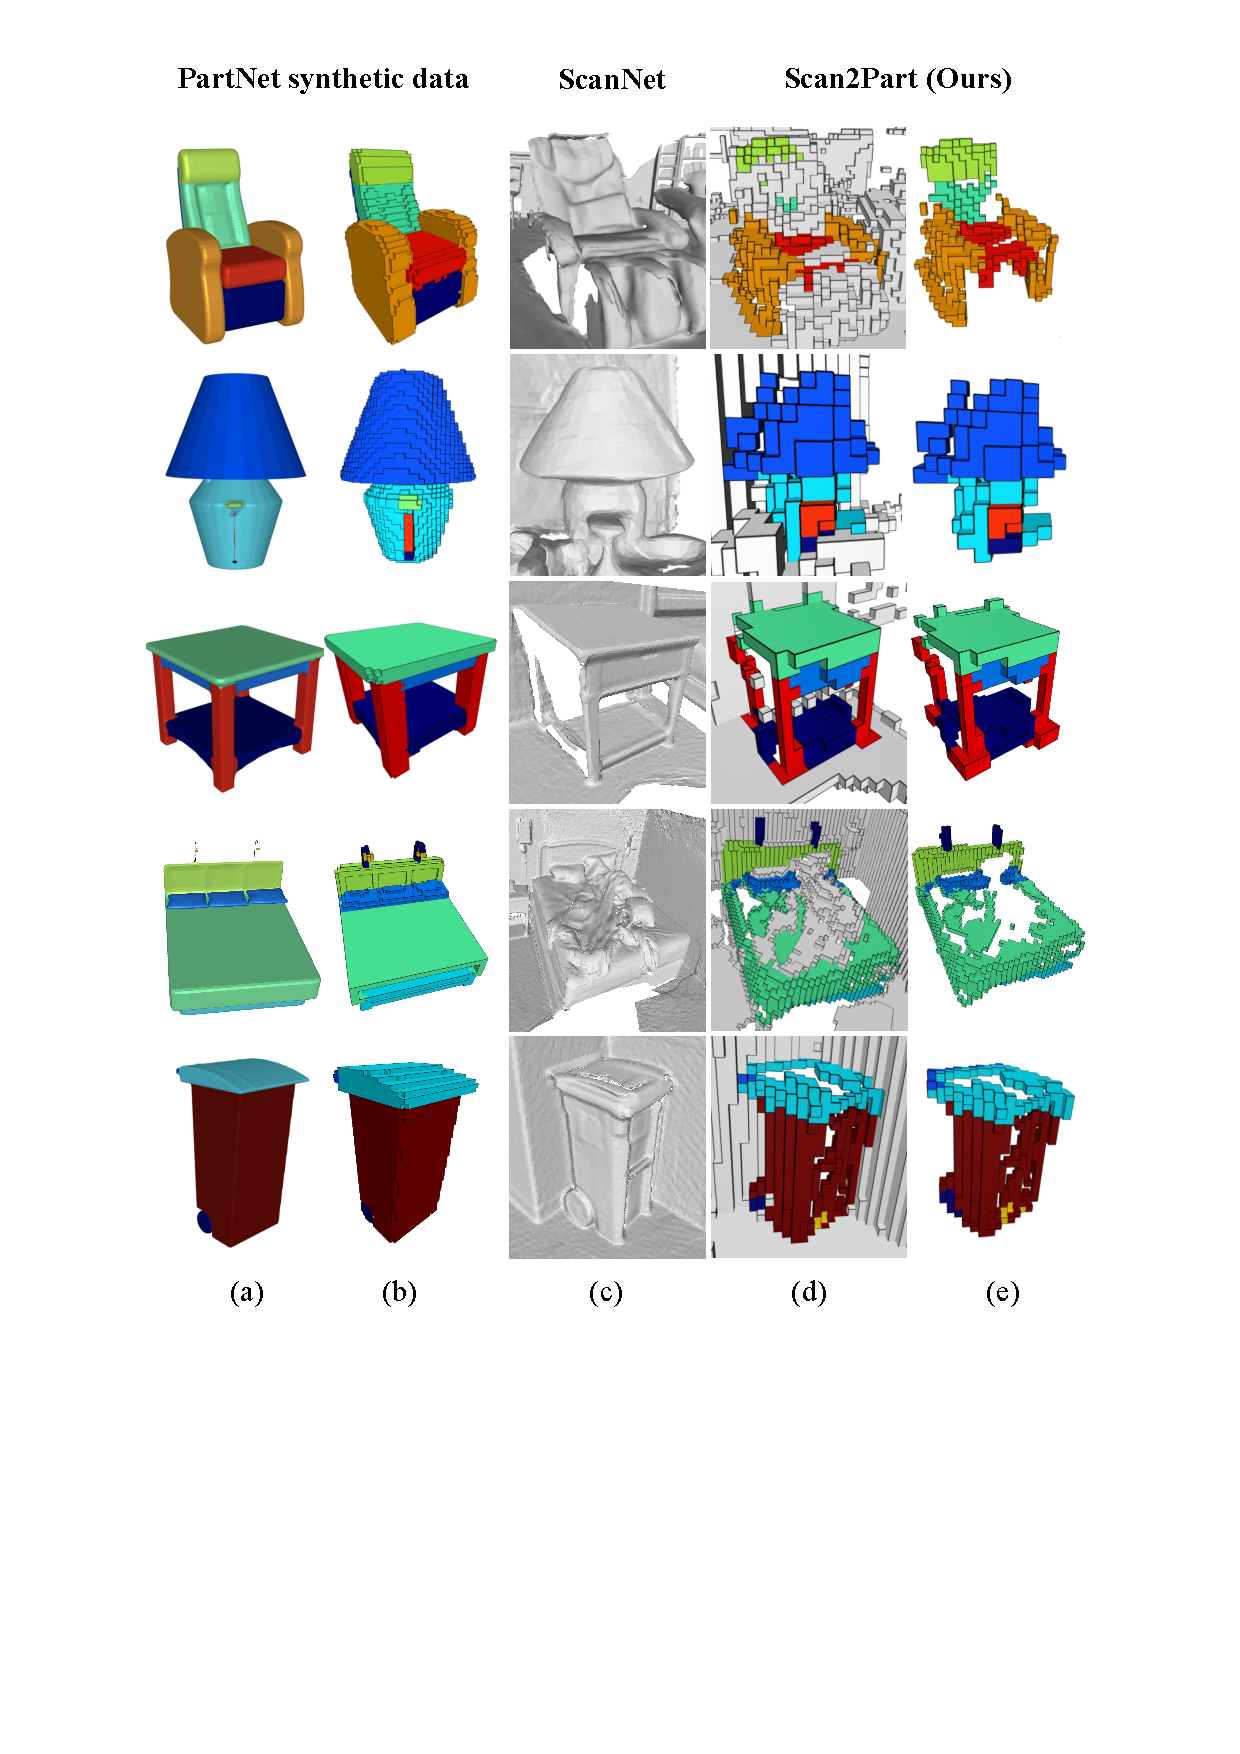
\includegraphics[width=\textwidth]{images/more_teasers.pdf}
\caption{Example voxelized shapes from our Scan2Part dataset. From left to right: 
(a) source 3D CAD model with part category annotations from PartNet~\cite{mo2019partnet},
(b) voxelized 3D shape with voxel-level parts annotation,
(c) fragment of reconstructed 3D scan geometry with a real-world instance of the same object,
(d) voxelized 3D scan geometry annotated according to our automatic procedure,
(e) real-world voxelized 3D shape (resolution $=3$\,cm$^3$) with voxel-level parts annotation.
Note the significant difference in geometry between synthetic and real-world volumetic 3D shapes due to noisy and incomplete geometry.}
\end{figure}


\begin{figure}[!t]
\label{fig:part_level_variation_voxels}
\centering
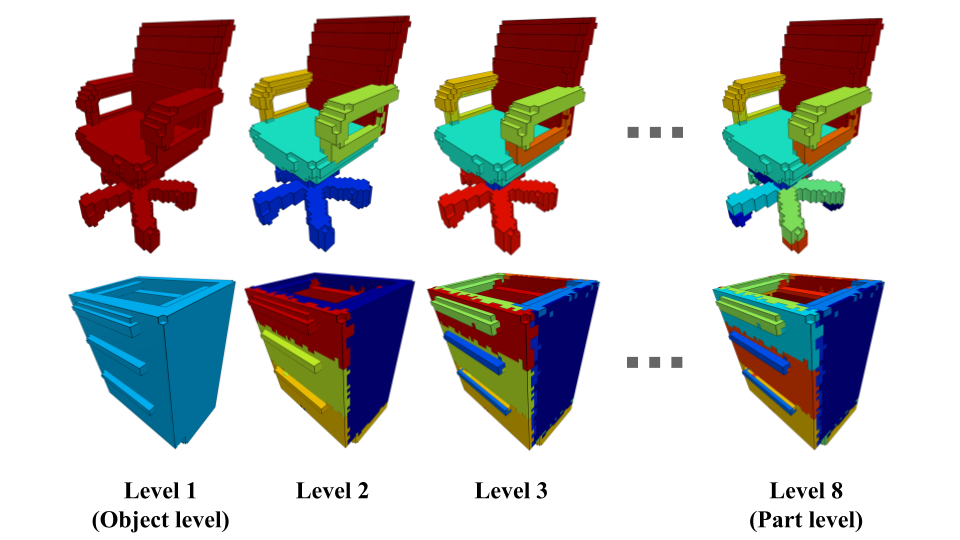
\includegraphics[width=\textwidth]{images/part_level_variation_voxels.png}
\caption{Example instances from our Scan2Part dataset, segmented according to level of detail depending on the part tree PartNet-based taxonomy~\cite{mo2019partnet}. The level of detail  increases from left to right, starting with the object level.}
\end{figure}

% \LA{figure displaying the taxonomy as a tree}
% VI: colored Treemap by AN

\begin{figure}[!t]
\label{fig:dataset_treemap}
\centering
% <left> <lower> <right> <upper>
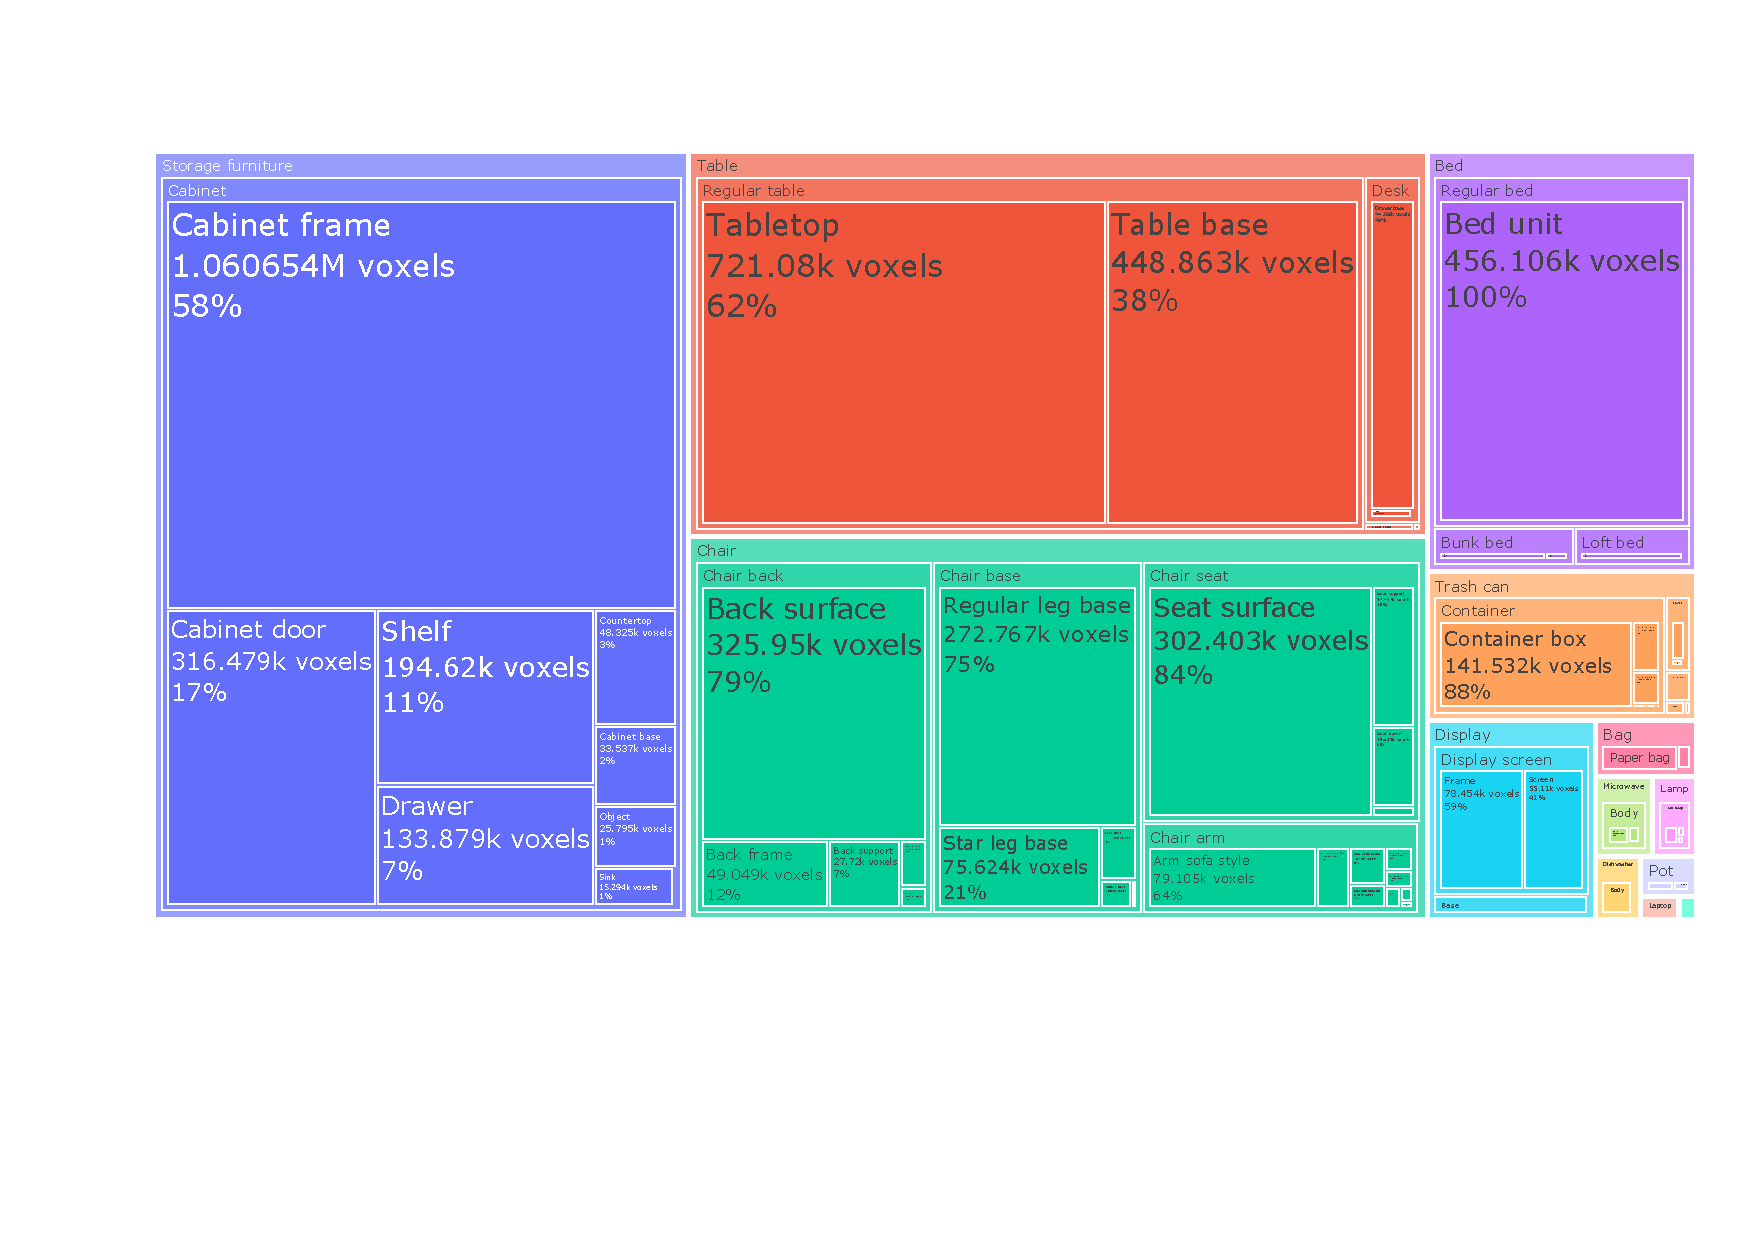
\includegraphics[trim={2.5cm 5cm 1cm 3cm},clip,width=\textwidth]{images/treemap_plot30px.pdf}
\caption{Statistics of Scan2Part dataset, area of tiles correspond to absolute number of voxels in the dataset}
\end{figure}


\paragraph{Dataset statistics. }
\label{dataset:statistics-detail}




% \begin{table}[!htb]
% \caption{Full dataset and testset statistics. As you can see it's highly unbalanced.}
% \resizebox{\textwidth}{!}{%
% \begin{tabular}{l|lllll}
% classes & \% in testset & \# voxel & \% voxels & \# scenes & \# inst. in testset\\ \hline
% Microwave & 18.75\% & 20141 & 0.38\% & 90 & 21\\
% Display & 19.36\% & 149988 & 2.84\% & 350 & 142\\
% Lamp & 20.14\% & 15736 & 0.30\% & 95 & 26\\
% Laptop & 19.95\% & 3950 & 0.07\% & 46 & 11\\
% Bag & 19.75\% & 25225 & 0.48\% & 136 & 33\\
% Storage & 19.41\% & 1833826 & 34.68\% & 866 & 496\\
% Bed & 20.94\% & 504774 & 9.55\% & 271 & 69\\
% Table & 20.82\% & 1268401 & 23.99\% & 1104 & 539\\
% Chair & 16.95\% & 1261928 & 23.87\% & 960 & 754\\
% Dishwasher & 20.99\% & 12846 & 0.24\% & 24 & 6\\
% TrashCan & 18.96\% & 178648 & 3.38\% & 634 & 199\\
% Vase & 20.48\% & 9989 & 0.19\% & 30 & 9\\
% Keyboard & 19.63\% & 1819 & 0.03\% & 24 & 9\\
% % Bowl & 28.86\% & 1178 & 0.02\% & 12 \\
% % Faucet & 2.44\% & 246 & 0.00\% & 4 \\
% % Clock & 12.28\% & 1742 & 0.03\% & 15 \\
% % Hat & 100.00\% & 101 & 0.00\% & 1 \\
% % Bottle & 0.00\% & 23 & 0.00\% & 1
% \end{tabular}%
% \label{tab:datasetstats}
% }
% \end{table}



% \begin{table}[hbt]
% \caption{Proportions of ShapeNet semantic classes present in Scan2Cad dataset}
% \label{table:scan2part_proportions}
% \begin{tabular}{l|l|l}
% Class ID & overlap? & class name \\
% \hline
% 04379243 & 99.0\% (822/830) & table \\ \hline
% 02747177 & 98.9\% (88/89) & ashcan,trash can,garbage can,wastebin,ash bin,ash-bin \\ \hline
% 03211117 & 97.6\% (161/165) & display,video display \\ \hline
% 03761084 & 97.3\% (36/37) & microwave,microwave oven \\ \hline
% 03337140 & 97.1\% (68/70) & file,file cabinet,filing cabinet \\ \hline
% 03001627 & 96.9\% (632/652) & chair \\ \hline
% 02871439 & 96.7\% (145/150) & bookshelf \\ \hline
% 02933112 & 94.8\% (294/310) & cabinet \\ \hline
% 02818832 & 94.0\% (47/50) & bed \\ \hline
% 03991062 & 91.7\% (11/12) & pot,flowerpot \\ \hline
% 03207941 & 85.7\% (12/14) & dishwasher,dish washer,dishwashing machine \\ \hline
% 03085013 & 81.8\% (9/11) & computer keyboard,keypad \\ \hline
% 03325088 & 57.1\% (4/7) & faucet,spigot \\ \hline
% 02876657 & 50.0\% (1/2) & bottle \\ \hline
% 02808440 & 26.0\% (25/96) & bathtub,bathing tub,bath,tub \\ \hline
% 02801938 & 9.4\% (3/32) & basket,handbasket \\ \hline
% 04256520 & 8.1\% (20/247) & sofa,couch,lounge \\ \hline
% 02946921 & 0.0\% (0/1) & can,tin,tin can \\ \hline
% 03938244 & 0.0\% (0/5) & pillow \\ \hline
% 02828884 & 0.0\% (0/28) & bench \\ \hline
% 04554684 & 0.0\% (0/37) & washer,automatic washer,washing machine \\ \hline
% 03928116 & 0.0\% (0/25) & piano,pianoforte,forte-piano \\ \hline
% 03790512 & 0.0\% (0/4) & motorcycle,bike \\ \hline
% 03691459 & 0.0\% (0/2) & loudspeaker,speaker,speaker unit,loudspeaker system \\ \hline
% 03467517 & 0.0\% (0/6) & guitar \\ \hline
% 04330267 & 0.0\% (0/36) & stove \\ \hline
% 04401088 & 0.0\% (0/1) & telephone,phone,telephone set \\ \hline
% 04004475 & 0.0\% (0/31) & printer,printing machine \\ \hline
% Total:    & 81.2\% (2477/3049) &         \\
% \end{tabular}
% \end{table}


\FloatBarrier
\clearpage

\section{Methodology details}
\label{supsec:methods-detail}



\paragraph{Architecture of our network. }
\label{methods:network-arch-detail}
The schematic depiction of our architecture is in Figure~\ref{fig:architecture}. Note that the architecture of the model varies slightly depending on the task (eg, on the number of predicted categories). 


\begin{figure}[!t]
\label{fig:architecture}
\centering
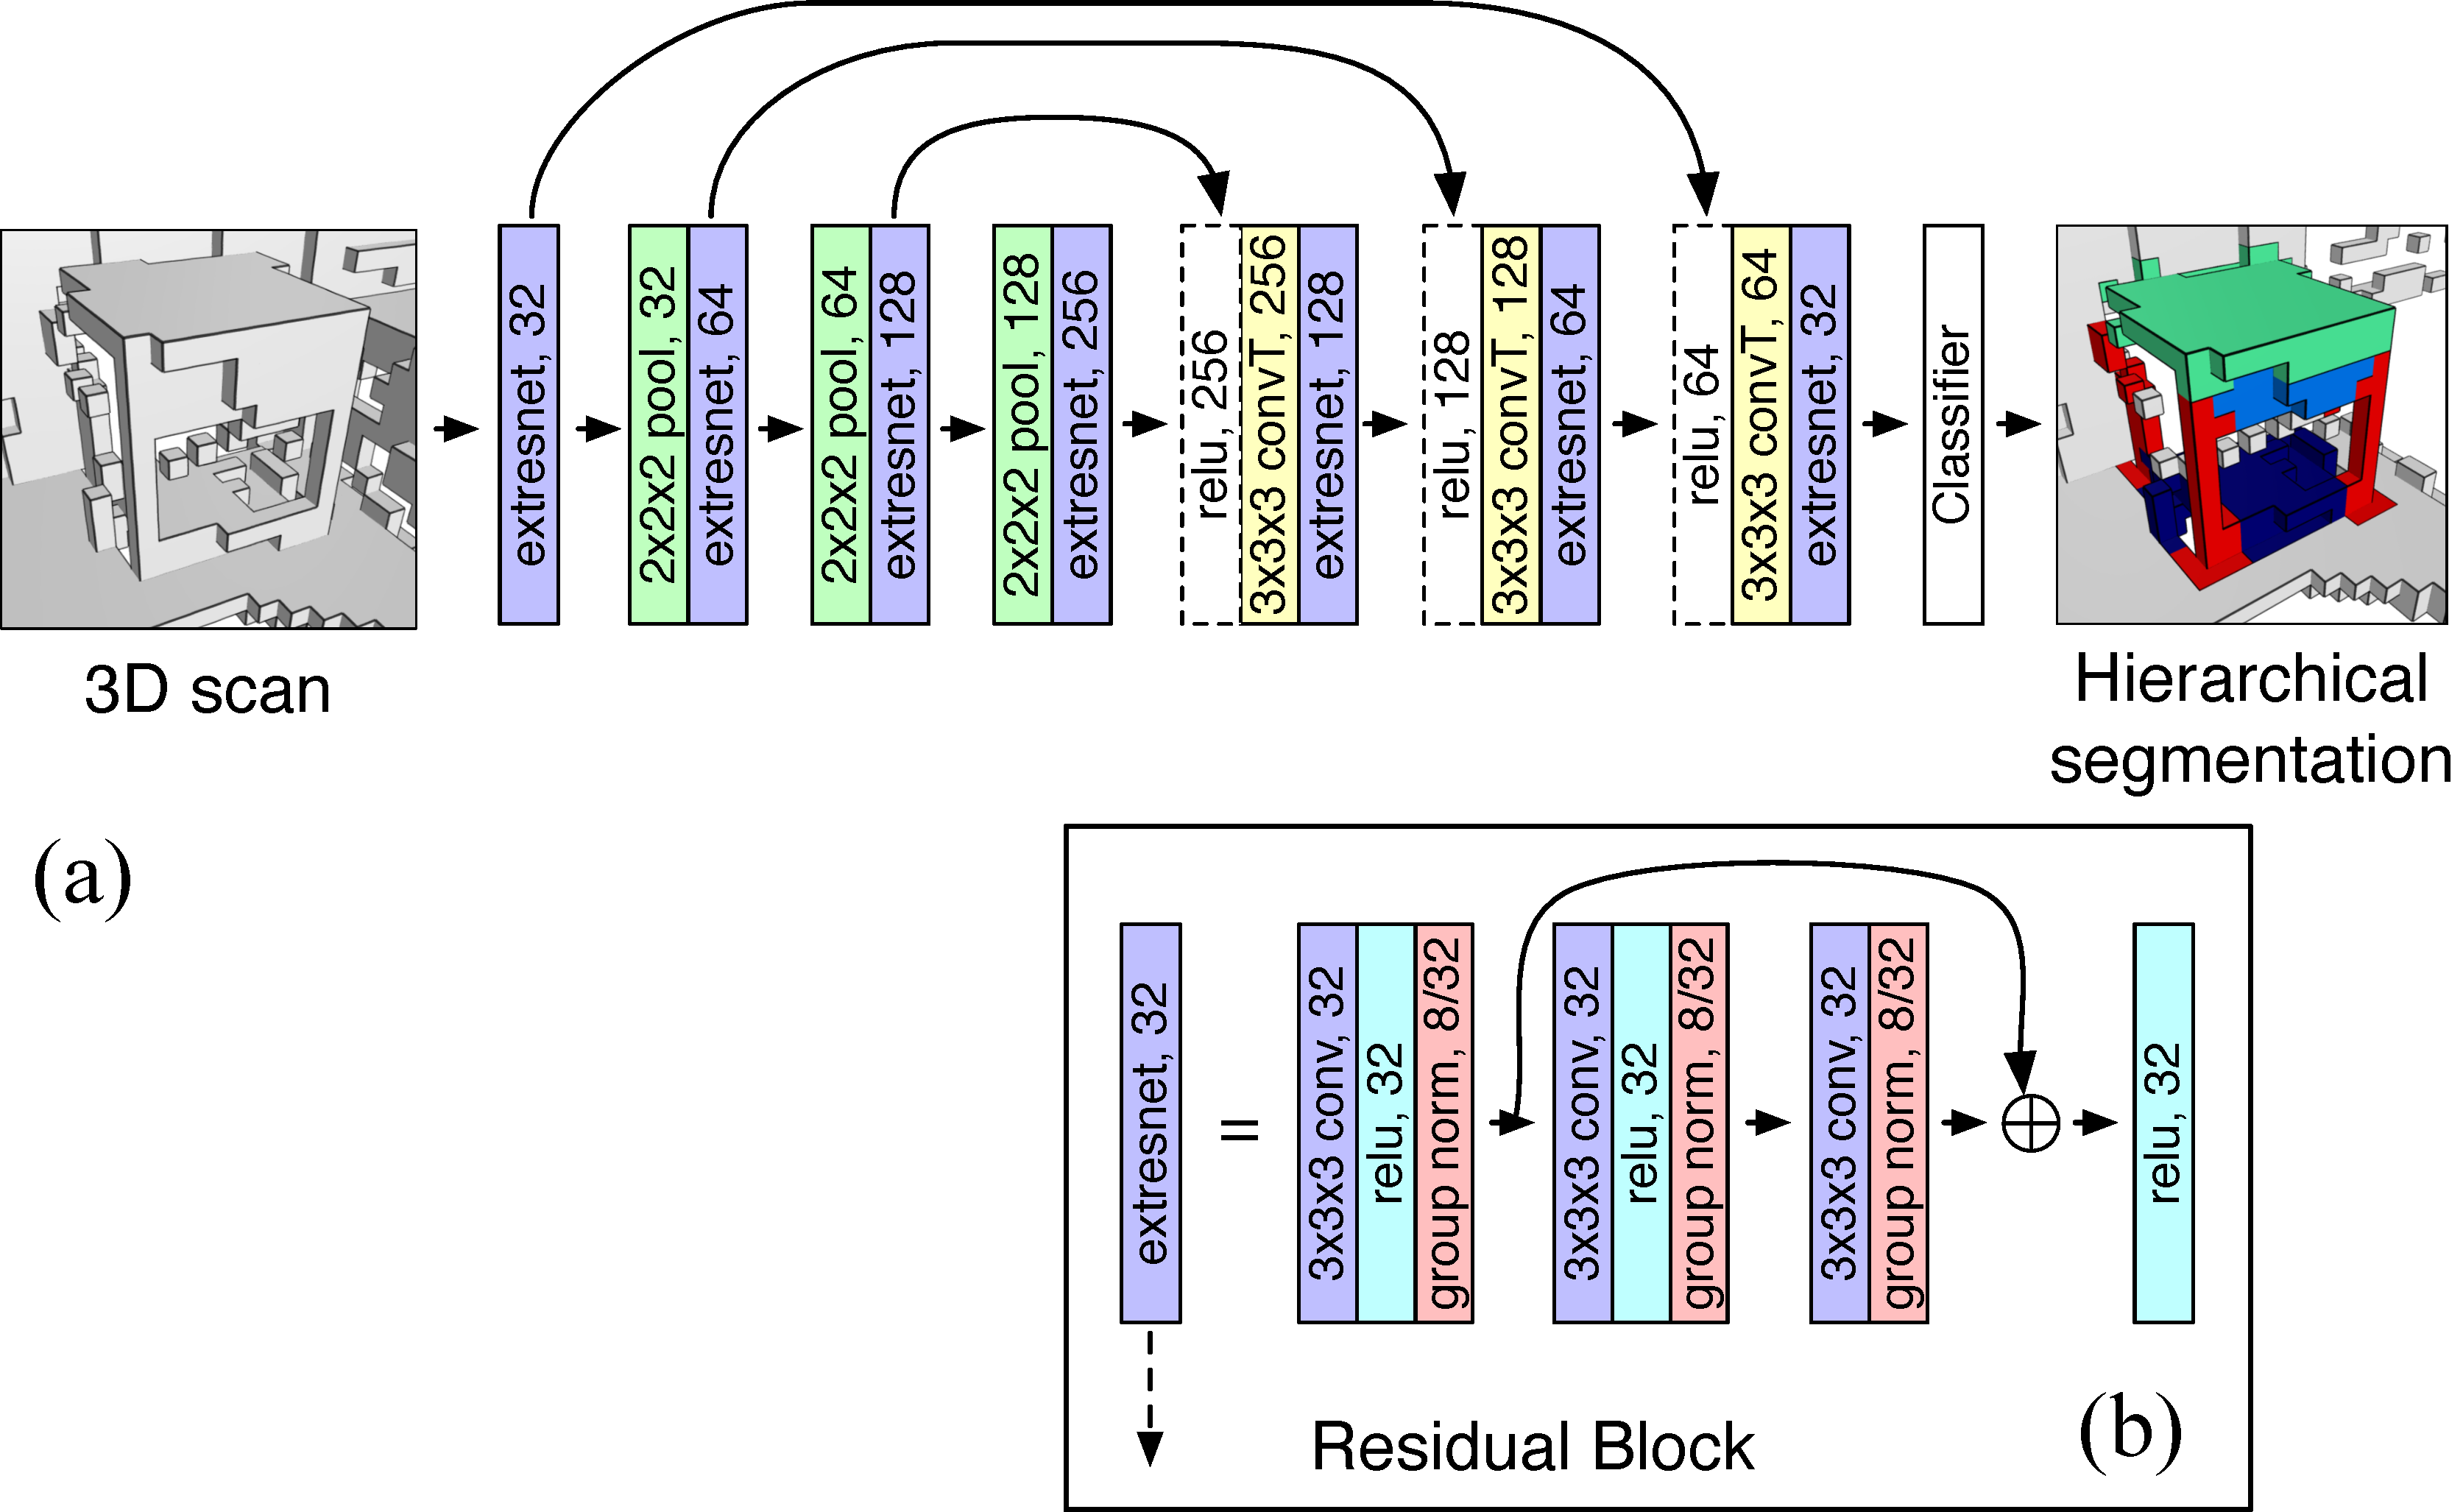
\includegraphics[width=0.9\textwidth]{images/scannet-unet3d-model-architecture}
\caption{The architecture of our model. Our architecture is a 3D U-net with residual blocks equipped with ReLU non-linearities and groupwise normalization layers. The model has 4 encoder and 3 decoder blocks with upsampling performed by transposed convolutions.}
\end{figure}



% \LA{figure displaying the architecture}


%  • [189] Specifically, as a backbone for our models we use a 3D version of the U-net architecture [57] with residual modules in both encoder and decoder branches (based on [58, 59]; see supplementary for a full network architecture) — здесь у нас есть картинка структуры сети, нужно ли что-то добавлять?

%  3. Визуализации архитектур, детальные для всех случаев. картинка структуры сети (есть одна из трёх) (отсылка к строке 189 основной статьи) 



\paragraph{Loss function for semantic instance segmentation. }
\label{methods:loss-detail}

To perform efficient voxel-wise instance segmentation, we opt to learn \emph{voxel embeddings} akin to \emph{pixel embeddings} in~\cite{de2017semantic}, aiming to cluster embeddings for the same object part together while pushing embeddings for separate parts farther apart.
To this end, we employ a multi-task loss function given by:
\begin{equation}
\label{eq:ours_instance_seg_loss}
L = \alpha_{\text{intra}} L_{\text{intra}}
  + \alpha_{\text{inter}} L_{\text{inter}}
  + \alpha_{\text{reg}} L_{\text{reg}}
  + \alpha_{\text{sep}} L_{\text{sep}}
\end{equation}
where 
$L_{\text{intra}}$ is an intra-part term aiming to pull embeddings of voxels with the same part ID closer together,
$L_{\text{inter}}$ is an inter-cluster term, pushing \emph{mean} voxel embeddings with distinct part IDs farther apart from each other,
$L_{\text{reg}}$ keeps the network activations bounded, thus acting as a regulartization term, and
$L_{\text{sep}}$ aims to enforce separation between objects and background representations in feature space. 
Constants $\alpha_{\text{intra}}, \alpha_{\text{inter}}$ are set to 1, and $\alpha_{\text{reg}}, \alpha_{\text{sep}}$ are set to 1e-3 in our evaluation. We evaluated Instance Segmentation with $L_{\text{sep}}$ only on coarse level of detail.
While the first three terms are identical to those in~\cite{de2017semantic,pham2019jsis3d}, the separation term $L_{\text{sep}}$ may be written down as:
\begin{equation}
\label{eq:ours_instance_seg_loss_sep_term}
L_{\text{sep}} = [\max_i|\mathbf{x}^{\text{fg}}_i - \mu|_1 - |\mathbf{x}^{\text{bg}}_i - \mu|_1 + \delta]_+
\end{equation}
where $\mathbf{x}^{\text{fg}}_i$ and $\mathbf{x}^{\text{bg}}_i$ are voxel embeddings for the part and background voxels, respectively, $\mu = \frac 1 N \sum_i \mathbf{x}^{\text{fg}}_i$ is the mean embedding for foreground voxels, and $\delta > 0$ is a hyper-parameter specifying the margin where the foreground-background separation force is active.









\FloatBarrier
\clearpage

\section{Detailed segmentation results}
\label{supsec:segmentation-detail}

% \paragraph{Specifications of our benchmarked networks. }
% \label{supsec:results:network-detail}



\subsection{Part-level semantic labeling}
\label{supsec:results:semantic-segmentation}

Please see more part-level semantic labeling results in Tables~\ref{suptbl:partseg-iou}--

% \AN{3 tables with class-wise results on part semantic segmentation for 3 different levels of detail}

\begin{table}[!h]
\caption{Coarse level mean IoU (\%)}
\centering
\begin{tabular}{lrrrrrrrr}
\toprule
 &  \multicolumn{2}{c}{Baseline} && \multicolumn{5}{c}{Multi-Task Training (MTT)} \\
 \cmidrule{2-3}
 \cmidrule{5-9}
Class 			  &  	 Coa. &  				Fin. &&  	12 &  		123-coa. &  		123-coa.\,ens. &  	  123-fin. &  123-fin.\,ens. \\
\midrule
Microwave         &       2.0 &                  6.7 &&     5.3 &             4.7 &                     5.8 &           8.0 &                   8.3 \\
Display           &      42.3 &                 28.9 &&    35.7 &            39.9 &                    39.5 &          39.0 &                  39.1 \\
Lamp              &      17.1 &                 11.4 &&    14.0 &            16.5 &                    13.7 &           9.6 &                   8.7 \\
Laptop            &       9.8 &                  5.6 &&     3.4 &            11.9 &                    10.4 &           6.9 &                   6.4 \\
Bag               &      10.0 &                  4.6 &&     6.8 &             7.4 &                     6.6 &           6.0 &                   6.1 \\
Storage\_furniture &      47.2 &                 40.6 &&    42.1 &            56.0 &                    55.3 &          44.3 &                  43.9 \\
Bed               &      32.0 &                 22.1 &&    36.9 &            32.7 &                    33.5 &          32.8 &                  33.2 \\
Table             &      49.2 &                 38.9 &&    47.4 &            46.1 &                    44.4 &          47.7 &                  46.6 \\
Chair             &      55.1 &                 50.3 &&    58.4 &            54.1 &                    53.7 &          62.0 &                  61.8 \\
Dishwasher        &       0.0 &                  0.2 &&     0.0 &             0.3 &                     0.2 &           0.0 &                   0.0 \\
Trash\_can         &      21.3 &                 18.8 &&    30.3 &            18.5 &                    19.3 &          25.8 &                  24.9 \\
Pot               &       1.8 &                  1.0 &&     1.7 &             2.7 &                     3.0 &           1.0 &                   1.1 \\
Keyboard          &       4.1 &                  1.2 &&     0.4 &            11.7 &                    10.8 &           1.3 &                   1.4 \\
\midrule
Mean              &      22.5 &                 17.7 &&    21.7 &            23.3 &                    22.8 &          21.9 &                  21.7 \\
\bottomrule
\end{tabular}
\label{suptbl:partseg-iou}
\end{table}


\begin{table}[!h]

\caption{Coarse level mAcc}
\centering
\begin{tabular}{lrrrrrrrr}
\toprule
 &  \multicolumn{2}{c}{Baseline} && \multicolumn{5}{c}{Multi-Task Training (MTT)} \\
 \cmidrule{2-3}
 \cmidrule{5-9}
Class 			  &  	 Coa. &  				Fin. &&  	12 &  		123-coa. &  		123-coa.\,ens. &  	  123-fin. &  123-fin.\,ens. \\
\midrule
Microwave         &       2.1 &                  9.7 &&     6.9 &             6.1 &                     8.4 &          11.6 &                  13.4 \\
Display           &      66.7 &                 56.0 &&    68.0 &            57.7 &                    58.7 &          67.7 &                  70.2 \\
Lamp              &      41.7 &                 55.3 &&    55.4 &            42.5 &                    44.7 &          48.5 &                  50.5 \\
Laptop            &      13.1 &                 16.8 &&     6.9 &            17.0 &                    17.6 &          11.3 &                  11.5 \\
Bag               &      41.4 &                 40.4 &&    40.3 &            46.1 &                    46.9 &          53.8 &                  53.8 \\
Storage\_furniture &      51.9 &                 44.3 &&    45.1 &            65.8 &                    64.4 &          48.5 &                  48.2 \\
Bed               &      50.1 &                 39.3 &&    56.6 &            50.2 &                    50.7 &          66.5 &                  63.6 \\
Table             &      74.3 &                 52.8 &&    67.7 &            71.7 &                    65.2 &          72.0 &                  67.6 \\
Chair             &      81.0 &                 86.7 &&    90.0 &            67.4 &                    73.0 &          70.7 &                  76.3 \\
Dishwasher        &       0.0 &                  0.3 &&     0.0 &             0.6 &                     0.5 &           0.0 &                   0.0 \\
Trash\_can         &      24.9 &                 21.9 &&    38.9 &            19.5 &                    21.5 &          31.9 &                  33.3 \\
Pot               &       8.6 &                  6.3 &&     8.2 &             7.9 &                     8.0 &           5.4 &                   5.6 \\
Keyboard          &       6.7 &                  4.2 &&     0.6 &            16.2 &                    18.8 &           2.8 &                   3.4 \\
\midrule
Mean              &      62.6 &                 54.2 &&    61.6 &            63.5 &                    62.8 &          60.7 &                  60.5 \\
\bottomrule
\end{tabular}
\end{table}


\begin{table}[!h]

\caption{middle level mIoU}
\centering
\begin{tabular}{lrrrrrrrr}
\toprule
 &  \multicolumn{2}{c}{Baseline} && \multicolumn{5}{c}{Multi-Task Training (MTT)} \\
 \cmidrule{2-3}
 \cmidrule{5-9}
Class 			  &  	 Mid. &  				Fin. &&  	12 &  		123-coa. &  		123-coa.\,ens. &  	  123-fin. &  123-fin.\,ens. \\
\midrule
Microwave/body           &              1.8 &                  6.7 &&     5.4 &             5.2 &                     5.9 &           8.1 &                   8.4 \\
Laptop/screen\_side       &             15.6 &                  9.2 &&     4.7 &            18.3 &                    16.1 &          10.2 &                  10.1 \\
Bag/luggage              &              4.1 &                  0.0 &&     0.5 &             0.0 &                     0.0 &           0.0 &                   0.0 \\
StorageFurniture/cabinet &             44.1 &                 40.2 &&    40.9 &            54.5 &                    55.0 &          40.9 &                  42.6 \\
Bed/regular\_bed          &             38.2 &                 22.0 &&    34.8 &            30.4 &                    33.1 &          31.3 &                  33.3 \\
Table/desk               &              9.2 &                  4.4 &&     7.0 &             5.2 &                     4.7 &           7.8 &                   8.1 \\
Table/regular\_table      &             49.9 &                 39.3 &&    47.3 &            44.0 &                    43.6 &          45.3 &                  45.2 \\
Chair/chair\_base         &             58.0 &                 45.9 &&    53.7 &            45.9 &                    41.8 &          54.2 &                  48.4 \\
Lamp/table\_lamp          &              1.9 &                  5.3 &&    14.4 &             3.7 &                     5.4 &           2.9 &                   4.5 \\
Dishwasher/body          &              0.0 &                  0.2 &&     0.0 &             0.2 &                     0.2 &           0.0 &                   0.0 \\
TrashCan/outside\_frame   &              0.0 &                  0.0 &&     1.4 &             0.0 &                     0.0 &           0.0 &                   0.0 \\
Chair/chair\_arm          &             18.9 &                 11.2 &&    13.0 &            12.7 &                    11.7 &          17.5 &                  15.9 \\
Bed/bunk\_bed             &              2.2 &                  0.9 &&    13.8 &             1.2 &                     1.9 &           1.5 &                   1.9 \\
Chair/chair\_seat         &             50.5 &                 36.9 &&    50.2 &            43.6 &                    38.6 &          47.6 &                  44.1 \\
TrashCan/container       &             34.2 &                 21.7 &&    30.9 &            21.2 &                    21.1 &          28.4 &                  28.7 \\
Vase/containing\_things   &              0.9 &                  1.5 &&     2.1 &             3.3 &                     3.9 &           1.0 &                   1.2 \\
Bag/hand\_or\_shoulder\_bag &              2.6 &                  1.3 &&     1.9 &             2.3 &                     2.2 &           2.0 &                   2.3 \\
Lamp/floor\_lamp          &              0.0 &                 19.3 &&     0.0 &             0.8 &                    20.2 &           1.0 &                  11.3 \\
StorageFurniture/chest   &              1.1 &                  0.3 &&     1.5 &             0.8 &                     0.6 &           1.0 &                   1.0 \\
Table/game\_table         &              0.0 &                  0.0 &&     0.0 &             0.6 &                     0.8 &           7.4 &                   5.6 \\
Laptop/base\_side         &              0.0 &                  0.0 &&     0.0 &             0.0 &                     0.6 &           0.0 &                   0.0 \\
TrashCan/cover           &              5.6 &                  1.3 &&     5.2 &             2.0 &                     1.8 &           4.1 &                   3.4 \\
Chair/chair\_back         &             50.0 &                 28.6 &&    39.6 &            38.8 &                    36.4 &          45.5 &                  42.8 \\
Display/base             &             11.5 &                  8.9 &&     9.3 &            10.9 &                    11.0 &          10.2 &                  10.9 \\
Vase/base                &              0.0 &                  0.0 &&     0.0 &             0.0 &                     0.0 &           0.0 &                   0.0 \\
Bag/paper\_bag            &              7.0 &                  3.6 &&     5.1 &             5.6 &                     4.4 &           5.3 &                   5.0 \\
TrashCan/base            &              7.1 &                  2.0 &&     1.3 &             0.0 &                     0.0 &           1.6 &                   1.6 \\
Display/display\_screen   &             41.5 &                 29.6 &&    35.5 &            41.1 &                    43.1 &          40.4 &                  42.5 \\
Chair/chair\_head         &              0.2 &                  0.2 &&     0.7 &             0.2 &                     0.4 &           0.5 &                   0.5 \\
Keyboard/frame           &              0.1 &                  0.8 &&     0.5 &             4.3 &                     5.2 &           0.5 &                   0.7 \\
Dishwasher/base          &              0.0 &                  0.0 &&     0.0 &             0.0 &                     0.0 &           0.0 &                   0.0 \\
Bed/loft\_bed             &              0.0 &                  1.9 &&     2.4 &             0.0 &                     0.0 &           0.0 &                   0.8 \\
TrashCan/other           &              0.0 &                  0.0 &&     0.0 &             0.0 &                     0.0 &           0.0 &                   0.0 \\
Vase/body                &              0.1 &                  0.4 &&     0.1 &             0.0 &                     0.0 &           0.1 &                   0.3 \\
Microwave/base           &              0.0 &                  0.0 &&     0.0 &             0.0 &                     0.0 &           0.0 &                   0.0 \\
Keyboard/key             &              0.0 &                  0.0 &&     0.0 &            14.9 &                    13.9 &           5.9 &                   5.9 \\
\midrule
Mean                     &             12.7 &                  9.5 &&    11.8 &            11.4 &                    11.8 &          11.7 &                  11.9 \\
\bottomrule
\end{tabular}
\end{table}

% --------------------------------------------------------------

\begin{table}[!h]

\caption{middle level mAcc}
\centering
\begin{tabular}{lrrrrrrrr}
\toprule
 &  \multicolumn{2}{c}{Baseline} && \multicolumn{5}{c}{Multi-Task Training (MTT)} \\
 \cmidrule{2-3}
 \cmidrule{5-9}
Class 			  &  	 Mid. &  				Fin. &&  	12 &  		123-coa. &  		123-coa.\,ens. &  	  123-fin. &  123-fin.\,ens. \\
\midrule
Microwave/body           &              2.1 &                  9.8 &&     6.8 &             6.7 &                     8.6 &          11.6 &                  13.6 \\
Laptop/screen\_side       &             19.2 &                 29.6 &&    12.2 &            30.2 &                    30.7 &          19.4 &                  20.3 \\
Bag/luggage              &             49.0 &                  0.0 &&     3.9 &             0.0 &                     0.0 &           0.0 &                   0.0 \\
StorageFurniture/cabinet &             48.1 &                 43.7 &&    43.7 &            63.0 &                    63.9 &          44.3 &                  46.7 \\
Bed/regular\_bed          &             64.0 &                 39.1 &&    56.2 &            47.3 &                    50.0 &          64.3 &                  63.5 \\
Table/desk               &             21.5 &                  9.1 &&    25.1 &            13.0 &                     8.8 &          29.3 &                  21.0 \\
Table/regular\_table      &             65.8 &                 52.5 &&    63.3 &            64.8 &                    64.8 &          61.3 &                  64.6 \\
Chair/chair\_base         &             80.8 &                 76.9 &&    76.6 &            58.9 &                    54.3 &          64.4 &                  58.4 \\
Lamp/table\_lamp          &             36.2 &                 47.7 &&    54.8 &            26.5 &                    30.8 &          35.6 &                  39.4 \\
Dishwasher/body          &              0.0 &                  0.4 &&     0.0 &             0.4 &                     0.5 &           0.0 &                   0.0 \\
TrashCan/outside\_frame   &              0.0 &                  0.0 &&     1.9 &             0.0 &                     0.0 &           0.0 &                   0.0 \\
Chair/chair\_arm          &             55.3 &                 54.6 &&    54.9 &            41.9 &                    43.8 &          44.5 &                  46.4 \\
Bed/bunk\_bed             &              4.9 &                  2.3 &&    20.5 &             3.8 &                     5.1 &           8.7 &                   6.0 \\
Chair/chair\_seat         &             76.9 &                 69.8 &&    78.5 &            60.0 &                    54.5 &          65.0 &                  61.1 \\
TrashCan/container       &             48.5 &                 24.5 &&    39.1 &            22.7 &                    23.4 &          35.0 &                  35.9 \\
Vase/containing\_things   &              4.2 &                  6.3 &&     9.3 &            11.3 &                    11.8 &           5.6 &                   6.2 \\
Bag/hand\_or\_shoulder\_bag &             16.3 &                 18.3 &&    18.0 &            30.3 &                    29.0 &          18.0 &                  18.4 \\
Lamp/floor\_lamp          &              0.0 &                 51.2 &&     0.0 &             0.9 &                    41.2 &           1.2 &                  47.7 \\
StorageFurniture/chest   &              4.1 &                  1.2 &&    10.1 &             5.0 &                     2.6 &           9.8 &                   6.6 \\
Table/game\_table         &              0.0 &                  0.0 &&     0.0 &             1.3 &                     1.6 &          32.4 &                  15.0 \\
Laptop/base\_side         &              0.0 &                  0.0 &&     0.0 &             0.0 &                     0.9 &           0.0 &                   0.0 \\
TrashCan/cover           &              8.0 &                  1.8 &&     9.9 &             2.3 &                     2.0 &           7.3 &                   5.8 \\
Chair/chair\_back         &             65.3 &                 39.8 &&    55.7 &            48.2 &                    45.8 &          53.7 &                  51.6 \\
Display/base             &             40.6 &                 33.1 &&    52.5 &            48.9 &                    47.4 &          59.6 &                  57.8 \\
Vase/base                &              0.0 &                  0.0 &&     0.0 &             0.0 &                     0.0 &           0.0 &                   0.0 \\
Bag/paper\_bag            &             46.3 &                 29.0 &&    28.0 &            24.5 &                    28.2 &          44.8 &                  45.8 \\
TrashCan/base            &             10.7 &                  6.3 &&     4.7 &             0.0 &                     0.0 &           6.7 &                   6.3 \\
Display/display\_screen   &             64.0 &                 53.6 &&    58.2 &            53.7 &                    53.9 &          61.6 &                  64.1 \\
Chair/chair\_head         &              1.5 &                  3.9 &&    10.7 &             2.4 &                     4.9 &           2.4 &                   2.9 \\
Keyboard/frame           &              0.3 &                  2.8 &&     0.7 &             6.6 &                     9.1 &           1.4 &                   1.7 \\
Dishwasher/base          &              0.0 &                  0.0 &&     0.0 &             0.0 &                     0.0 &           0.0 &                   0.0 \\
Bed/loft\_bed             &              0.0 &                  4.4 &&     3.0 &             0.0 &                     0.0 &           0.0 &                   1.4 \\
TrashCan/other           &              0.0 &                  0.0 &&     0.0 &             0.0 &                     0.0 &           0.0 &                   0.0 \\
Vase/body                &              0.3 &                  4.5 &&     0.3 &             0.0 &                     0.0 &           0.7 &                   1.5 \\
Microwave/base           &              0.0 &                  0.0 &&     0.0 &             0.0 &                     0.0 &           0.0 &                   0.0 \\
Keyboard/key             &              0.0 &                  0.0 &&     0.0 &            26.1 &                    27.5 &           8.7 &                   8.7 \\
\midrule
Mean                     &             57.9 &                 47.1 &&    53.5 &            56.2 &                    56.1 &          52.6 &                  53.5 \\
\bottomrule
\end{tabular}
\end{table}

% --------------------------------------------------------------

\begin{table}[!h]
\caption{fine level mIoU}
\centering
\begin{tabular}{lrrrrr}
\toprule
 &  \multicolumn{1}{c}{Baseline} & \multicolumn{4}{c}{Multi-Task Training (MTT)} \\
 \cmidrule{3-6}
Class 			  &  	 Fin. &  	123-coa. &  		123-coa.\,ens. &  	  123-fin. &  123-fin.\,ens. \\
\midrule
Bowl/container                 &            0.0 &             4.4 &                     0.0 &           0.0 &                   0.0 \\
Lamp/lamp\_unit                 &           19.3 &            20.1 &                     2.2 &          11.3 &                   4.7 \\
Laptop/screen                  &            1.7 &             2.8 &                     2.8 &          11.5 &                  10.7 \\
StorageFurniture/cabinet\_door  &           15.2 &            19.7 &                    19.9 &           5.9 &                   6.7 \\
Clock/clock\_body               &            0.4 &             0.6 &                     0.0 &           0.0 &                   0.0 \\
Bed/bed\_unit                   &           22.0 &            32.8 &                    32.4 &          33.3 &                  32.8 \\
StorageFurniture/cabinet\_frame &           12.5 &            10.9 &                    11.9 &          11.4 &                  12.2 \\
StorageFurniture/sink          &            1.9 &             5.9 &                     6.2 &           7.8 &                   7.4 \\
Table/drawer\_base              &            4.2 &             4.1 &                     4.7 &           8.1 &                   8.2 \\
StorageFurniture/drawer        &           10.2 &             6.6 &                     6.6 &           9.5 &                   8.9 \\
Table/table\_base               &           21.6 &            25.1 &                    24.8 &          29.2 &                  28.4 \\
Chair/regular\_leg\_base         &           26.9 &            17.9 &                    19.5 &          27.5 &                  28.9 \\
Microwave/frame                &            3.9 &             2.0 &                     2.2 &           4.4 &                   4.3 \\
Chair/arm\_holistic\_frame       &            1.2 &             0.8 &                     0.8 &           0.5 &                   0.6 \\
StorageFurniture/countertop    &           11.3 &            10.4 &                    10.4 &          10.5 &                   9.9 \\
Bed/ladder                     &            0.9 &             1.9 &                     2.0 &           1.9 &                   1.7 \\
Chair/seat\_surface             &           31.9 &            33.3 &                    34.5 &          34.5 &                  35.3 \\
TrashCan/container\_neck        &            9.9 &             8.3 &                     8.6 &          12.5 &                  12.1 \\
Chair/arm\_slant\_bar            &            0.5 &             0.5 &                     0.7 &           0.2 &                   0.2 \\
Chair/other                    &            0.1 &             0.0 &                     0.0 &           0.1 &                   0.4 \\
Chair/armrest\_hard\_surface     &            3.3 &             2.8 &                     3.0 &           5.0 &                   4.8 \\
Chair/star\_leg\_base            &           21.2 &            12.2 &                    12.2 &          16.4 &                  16.5 \\
Lamp/lamp\_body                 &            3.7 &             8.6 &                     5.2 &           7.0 &                   3.5 \\
Table/tabletop                 &           46.3 &            49.8 &                    51.6 &          50.9 &                  52.3 \\
Chair/foot\_base                &            2.5 &             2.2 &                     1.7 &           2.4 &                   2.2 \\
Chair/arm\_connector            &            2.9 &             1.2 &                     0.8 &           0.8 &                   0.6 \\
TrashCan/frame\_vertical\_bar    &            0.0 &             0.0 &                     0.0 &           0.0 &                   0.0 \\
Table/foosball\_table           &            0.0 &             0.9 &                     0.9 &           6.0 &                   7.4 \\
Vase/plant                     &            1.6 &             4.0 &                     3.6 &           1.2 &                   1.1 \\
Laptop/base\_frame              &            0.0 &             0.8 &                     0.0 &           0.0 &                   0.0 \\
Microwave/door                 &            0.5 &             0.7 &                     1.0 &           1.8 &                   1.7 \\
Laptop/keyboard                &            0.0 &             0.0 &                     0.0 &           0.0 &                   0.0 \\
TrashCan/cover\_frame           &            0.0 &             0.0 &                     0.0 &           0.0 &                   0.0 \\
Chair/arm\_horizontal\_bar       &            1.9 &             1.1 &                     1.5 &           2.9 &                   3.1 \\
Chair/back\_surface             &           20.7 &            23.7 &                    24.8 &          26.5 &                  28.1 \\
\bottomrule
\end{tabular}
\end{table}

\begin{table}[!h]
\caption{fine level mIoU}
\centering
\begin{tabular}{lrrrrr}
\toprule
 &  \multicolumn{1}{c}{Baseline} & \multicolumn{4}{c}{Multi-Task Training (MTT)} \\
 \cmidrule{3-6}
Class 			  &  	 Fin. &  	123-coa. &  		123-coa.\,ens. &  	  123-fin. &  123-fin.\,ens. \\
\midrule
Display/foot\_base              &            0.0 &             0.0 &                     0.0 &           0.0 &                   0.0 \\
Chair/back\_frame               &            4.6 &             4.1 &                     4.4 &           6.2 &                   6.7 \\
Chair/pedestal\_base            &            0.0 &             0.0 &                     0.0 &           0.0 &                   0.0 \\
Chair/arm\_vertical\_bar         &            3.6 &             3.6 &                     3.7 &           3.9 &                   4.1 \\
Display/surface\_base           &           10.3 &            12.1 &                    11.8 &          11.4 &                  11.3 \\
Bag/handle                     &            0.2 &             0.3 &                     0.4 &           0.5 &                   0.7 \\
Display/screen                 &           21.3 &            29.5 &                    29.4 &          24.1 &                  24.0 \\
TrashCan/container\_handle      &            0.0 &             0.0 &                     0.0 &           0.0 &                   0.0 \\
StorageFurniture/cabinet\_base  &            6.6 &             8.1 &                     7.7 &           7.8 &                   6.8 \\
StorageFurniture/mirror        &            0.0 &             0.0 &                     0.0 &           0.0 &                   0.0 \\
Chair/surface\_base             &            0.1 &             0.3 &                     0.3 &           1.4 &                   1.2 \\
Keyboard/frame                 &            0.8 &             5.2 &                     4.9 &           0.7 &                   1.2 \\
Chair/seat\_frame               &            6.3 &             6.1 &                     5.9 &           6.9 &                   6.5 \\
Lamp/lamp\_base                 &            3.5 &             1.9 &                     1.3 &           2.1 &                   1.8 \\
StorageFurniture/object        &            0.9 &             3.6 &                     3.5 &           2.9 &                   2.8 \\
Chair/back\_connector           &            3.3 &             2.8 &                     1.5 &           3.9 &                   1.9 \\
Chair/headrest                 &            0.2 &             0.3 &                     0.4 &           0.5 &                   0.5 \\
Dishwasher/surface\_base        &            0.0 &             0.0 &                     0.0 &           0.0 &                   0.0 \\
Microwave/side\_controls        &            0.6 &             0.6 &                     0.3 &           1.4 &                   1.1 \\
Display/frame                  &           11.7 &            16.6 &                    17.0 &          18.9 &                  18.5 \\
TrashCan/container\_basket      &            0.0 &             0.0 &                     0.0 &           0.0 &                   0.0 \\
TrashCan/wheel\_base            &            2.3 &             0.0 &                     0.0 &           1.7 &                   1.9 \\
TrashCan/frame\_holistic        &            0.0 &             0.0 &                     0.0 &           0.0 &                   0.0 \\
Chair/back\_support             &            3.7 &             3.9 &                     4.0 &           4.4 &                   4.4 \\
StorageFurniture/shelf         &           21.2 &            14.3 &                    14.2 &          18.2 &                  18.1 \\
Bag/bag\_body                   &            3.7 &             5.1 &                     5.3 &           5.0 &                   5.0 \\
Laptop/screen\_frame            &            5.6 &            10.2 &                    12.4 &           5.1 &                   5.7 \\
TrashCan/other\_leaf            &            0.0 &             0.0 &                     0.0 &           0.0 &                   0.0 \\
Vase/container                 &            0.4 &             0.0 &                     0.0 &           0.3 &                   0.1 \\
Chair/arm\_sofa\_style           &           10.5 &            11.3 &                    11.6 &          13.6 &                  14.2 \\
Table/hutch                    &            4.0 &             2.0 &                     1.8 &           1.4 &                   1.5 \\
Chair/armrest\_soft\_surface     &            0.3 &             0.8 &                     0.8 &           1.7 &                   1.9 \\
TrashCan/container\_bottom      &            8.8 &             7.2 &                     7.8 &           9.4 &                   9.4 \\
Bed/furniture                  &            1.8 &             0.0 &                     0.0 &           0.8 &                   0.0 \\
TrashCan/cover\_lid             &            1.8 &             2.0 &                     2.0 &           3.3 &                   3.3 \\
StorageFurniture/chest\_base    &            0.4 &             0.6 &                     0.7 &           1.0 &                   1.0 \\
Chair/arm\_writing\_table        &            0.0 &             0.0 &                     0.0 &           0.0 &                   0.0 \\
Dishwasher/frame               &            0.3 &             0.4 &                     0.4 &           0.0 &                   0.0 \\
Dishwasher/door                &            0.2 &             0.0 &                     0.0 &           0.0 &                   0.0 \\
Chair/pillow                   &            0.1 &             0.4 &                     0.4 &           1.2 &                   1.4 \\
Bag/shoulder\_strap             &            1.3 &             2.2 &                     2.3 &           2.3 &                   2.0 \\
TrashCan/container\_box         &           11.2 &             7.9 &                     8.6 &          14.9 &                  15.5 \\
Chair/seat\_support             &            6.1 &             6.5 &                     6.5 &           7.6 &                   7.5 \\
Keyboard/key                   &            0.0 &            13.8 &                    16.1 &           5.9 &                   5.1 \\
\midrule
Mean                           &            5.8 &             6.3 &                     6.1 &           6.7 &                   6.6 \\
\bottomrule
\end{tabular}
\end{table}

% --------------------------------------------------------------

\begin{table}[!h]
\caption{fine level mAcc}
\centering
\begin{tabular}{lrrrrr}
\toprule
 &  \multicolumn{1}{c}{Baseline} & \multicolumn{4}{c}{Multi-Task Training (MTT)} \\
 \cmidrule{3-6}
Class 			  &  	 Fin. &  	123-coa. &  		123-coa.\,ens. &  	  123-fin. &  123-fin.\,ens. \\
\midrule
Bowl/container                 &            0.0 &            10.8 &                     0.0 &           0.0 &                   0.0 \\
Lamp/lamp\_unit                 &           51.2 &            40.7 &                     2.3 &          47.7 &                   7.4 \\
Laptop/screen                  &            2.3 &             3.0 &                     3.0 &          16.7 &                  15.2 \\
StorageFurniture/cabinet\_door  &           18.6 &            26.2 &                    26.9 &           6.5 &                   7.5 \\
Clock/clock\_body               &           12.6 &            24.8 &                     0.0 &           0.9 &                   0.0 \\
Bed/bed\_unit                   &           39.0 &            49.1 &                    49.8 &          63.4 &                  65.8 \\
StorageFurniture/cabinet\_frame &           13.8 &            12.2 &                    13.6 &          12.5 &                  13.5 \\
StorageFurniture/sink          &            5.4 &            41.3 &                    41.3 &          23.9 &                  20.3 \\
Table/drawer\_base              &            8.5 &             7.0 &                     9.5 &          20.7 &                  25.1 \\
StorageFurniture/drawer        &           16.5 &             8.5 &                     8.5 &          14.0 &                  12.8 \\
Table/table\_base               &           34.3 &            51.4 &                    51.3 &          51.7 &                  48.5 \\
Chair/regular\_leg\_base         &           38.4 &            21.1 &                    23.5 &          31.9 &                  34.2 \\
Microwave/frame                &            6.1 &             2.9 &                     3.0 &           7.3 &                   6.7 \\
Chair/arm\_holistic\_frame       &            2.9 &             4.4 &                     3.4 &           1.9 &                   1.5 \\
StorageFurniture/countertop    &           19.5 &            26.7 &                    26.2 &          27.8 &                  25.2 \\
Bed/ladder                     &            2.3 &             5.1 &                     5.6 &           6.0 &                   5.9 \\
Chair/seat\_surface             &           45.9 &            40.2 &                    43.0 &          41.2 &                  43.0 \\
TrashCan/container\_neck        &           18.9 &            25.7 &                    22.1 &          40.9 &                  33.9 \\
Chair/arm\_slant\_bar            &            6.5 &             3.9 &                     3.6 &           0.6 &                   0.6 \\
Chair/other                    &            1.5 &             0.0 &                     0.0 &           1.5 &                   1.5 \\
Chair/armrest\_hard\_surface     &           23.9 &            13.5 &                    11.7 &          15.5 &                  11.8 \\
Chair/star\_leg\_base            &           58.0 &            17.3 &                    17.3 &          22.6 &                  22.7 \\
Lamp/lamp\_body                 &           30.6 &            22.6 &                    23.0 &          24.8 &                  26.8 \\
Table/tabletop                 &           57.5 &            62.0 &                    66.3 &          65.5 &                  68.6 \\
Chair/foot\_base                &           23.4 &            26.9 &                    19.5 &          22.2 &                  17.0 \\
Chair/arm\_connector            &           14.6 &             6.0 &                     2.3 &           3.7 &                   1.6 \\
TrashCan/frame\_vertical\_bar    &            0.0 &             0.0 &                     0.0 &           0.0 &                   0.0 \\
Table/foosball\_table           &            0.0 &             1.9 &                     1.9 &          18.0 &                  27.8 \\
Vase/plant                     &            6.6 &            12.4 &                    12.2 &           6.6 &                   6.6 \\
Laptop/base\_frame              &            0.0 &             1.2 &                     0.0 &           0.0 &                   0.0 \\
Microwave/door                 &            0.6 &             0.8 &                     1.1 &           3.1 &                   2.6 \\
Laptop/keyboard                &            0.0 &             0.0 &                     0.0 &           0.0 &                   0.0 \\
TrashCan/cover\_frame           &            0.0 &             0.0 &                     0.0 &           0.0 &                   0.0 \\
Chair/arm\_horizontal\_bar       &           22.3 &             7.4 &                     7.1 &          16.9 &                  12.6 \\
Chair/back\_surface             &           26.8 &            27.6 &                    29.4 &          30.7 &                  32.9 \\
\bottomrule
\end{tabular}
\end{table}

\begin{table}[!h]
\caption{fine level mAcc}
\centering
\begin{tabular}{lrrrrr}
\toprule
 &  \multicolumn{1}{c}{Baseline} & \multicolumn{4}{c}{Multi-Task Training (MTT)} \\
 \cmidrule{3-6}
Class 			  &  	 Fin. &  	123-coa. &  		123-coa.\,ens. &  	  123-fin. &  123-fin.\,ens. \\
\midrule
Display/foot\_base              &            0.0 &             0.0 &                     0.0 &           0.0 &                   0.0 \\
Chair/back\_frame               &           13.3 &             8.3 &                     8.9 &          12.5 &                  13.5 \\
Chair/pedestal\_base            &            0.0 &             0.0 &                     0.0 &           0.0 &                   0.0 \\
Chair/arm\_vertical\_bar         &           19.7 &            13.9 &                    10.8 &          14.5 &                  12.1 \\
Display/surface\_base           &           33.2 &            47.5 &                    46.0 &          58.0 &                  57.8 \\
Bag/handle                     &            5.9 &            23.0 &                    17.1 &          10.5 &                  10.5 \\
Display/screen                 &           42.4 &            42.6 &                    42.8 &          37.1 &                  37.2 \\
TrashCan/container\_handle      &            0.0 &             0.0 &                     0.0 &           0.0 &                   0.0 \\
StorageFurniture/cabinet\_base  &           15.1 &            33.9 &                    29.5 &          23.7 &                  18.9 \\
StorageFurniture/mirror        &            0.0 &             0.0 &                     0.0 &           0.0 &                   0.0 \\
Chair/surface\_base             &            0.9 &             0.7 &                     0.7 &           2.6 &                   2.0 \\
Keyboard/frame                 &            2.8 &             9.1 &                     7.3 &           1.7 &                   3.1 \\
Chair/seat\_frame               &           31.9 &            26.9 &                    25.9 &          24.9 &                  24.1 \\
Lamp/lamp\_base                 &           34.9 &            15.6 &                    11.7 &          27.4 &                  24.8 \\
StorageFurniture/object        &            1.7 &            44.8 &                    45.5 &          30.1 &                  30.7 \\
Chair/back\_connector           &            7.5 &             6.1 &                     2.6 &           6.7 &                   3.0 \\
Chair/headrest                 &            3.9 &             4.9 &                     4.4 &           2.9 &                   2.4 \\
Dishwasher/surface\_base        &            0.0 &             0.0 &                     0.0 &           0.0 &                   0.0 \\
Microwave/side\_controls        &            1.7 &             6.8 &                     1.7 &           5.1 &                   3.4 \\
Display/frame                  &           23.8 &            23.8 &                    26.0 &          35.8 &                  36.3 \\
TrashCan/container\_basket      &            0.0 &             0.0 &                     0.0 &           0.0 &                   0.0 \\
TrashCan/wheel\_base            &            9.1 &             0.0 &                     0.0 &           9.1 &                   9.1 \\
TrashCan/frame\_holistic        &            0.0 &             0.0 &                     0.0 &           0.0 &                   0.0 \\
Chair/back\_support             &            6.8 &             6.3 &                     6.7 &           9.5 &                   9.8 \\
StorageFurniture/shelf         &           46.2 &            38.1 &                    38.1 &          32.8 &                  32.6 \\
Bag/bag\_body                   &           27.7 &            20.9 &                    21.4 &          43.3 &                  43.9 \\
Laptop/screen\_frame            &           23.5 &            24.8 &                    24.4 &          11.9 &                  12.2 \\
TrashCan/other\_leaf            &            0.0 &             0.0 &                     0.0 &           0.0 &                   0.0 \\
Vase/container                 &            4.5 &             0.0 &                     0.0 &           1.5 &                   0.8 \\
Chair/arm\_sofa\_style           &           40.0 &            32.8 &                    33.7 &          33.9 &                  35.5 \\
Table/hutch                    &           20.6 &            19.5 &                    10.7 &           7.6 &                   5.7 \\
Chair/armrest\_soft\_surface     &            1.8 &             7.6 &                     5.6 &          12.2 &                   9.0 \\
TrashCan/container\_bottom      &           31.0 &            14.7 &                    16.1 &          39.7 &                  39.5 \\
Bed/furniture                  &            4.3 &             0.0 &                     0.0 &           1.4 &                   0.0 \\
TrashCan/cover\_lid             &            2.0 &             2.2 &                     2.2 &           5.6 &                   5.5 \\
StorageFurniture/chest\_base    &            2.1 &             3.9 &                     5.5 &          11.0 &                  11.5 \\
Chair/arm\_writing\_table        &            NaN &             NaN &                     NaN &           NaN &                   NaN \\
Dishwasher/frame               &            0.6 &             1.3 &                     1.2 &           0.0 &                   0.0 \\
Dishwasher/door                &            0.2 &             0.0 &                     0.0 &           0.0 &                   0.0 \\
Chair/pillow                   &            0.8 &            14.7 &                    13.3 &          31.4 &                  26.0 \\
Bag/shoulder\_strap             &           18.3 &            28.9 &                    29.1 &          18.4 &                  17.6 \\
TrashCan/container\_box         &           11.7 &             8.1 &                     8.9 &          16.2 &                  17.3 \\
Chair/seat\_support             &           31.6 &            13.9 &                    12.8 &          24.2 &                  22.2 \\
Keyboard/key                   &            0.0 &            27.5 &                    26.1 &           8.7 &                   7.2 \\
\midrule
Mean                           &           31.0 &            32.5 &                    33.8 &          34.7 &                  35.6 \\
\bottomrule
\end{tabular}
\end{table}


\paragraph{Qualitative semantic labeling results}
\label{supsec:results:semantic-segmentation-qualitative}

% \VI{DONE: add figure with more visualizations}
%  6. Несколько дополнительных результатов работы алгоритма (нет) (наподобие рисунка 4 основной статьи)

\begin{figure}[!t]
\label{fig:semantic_experiments}
\centering
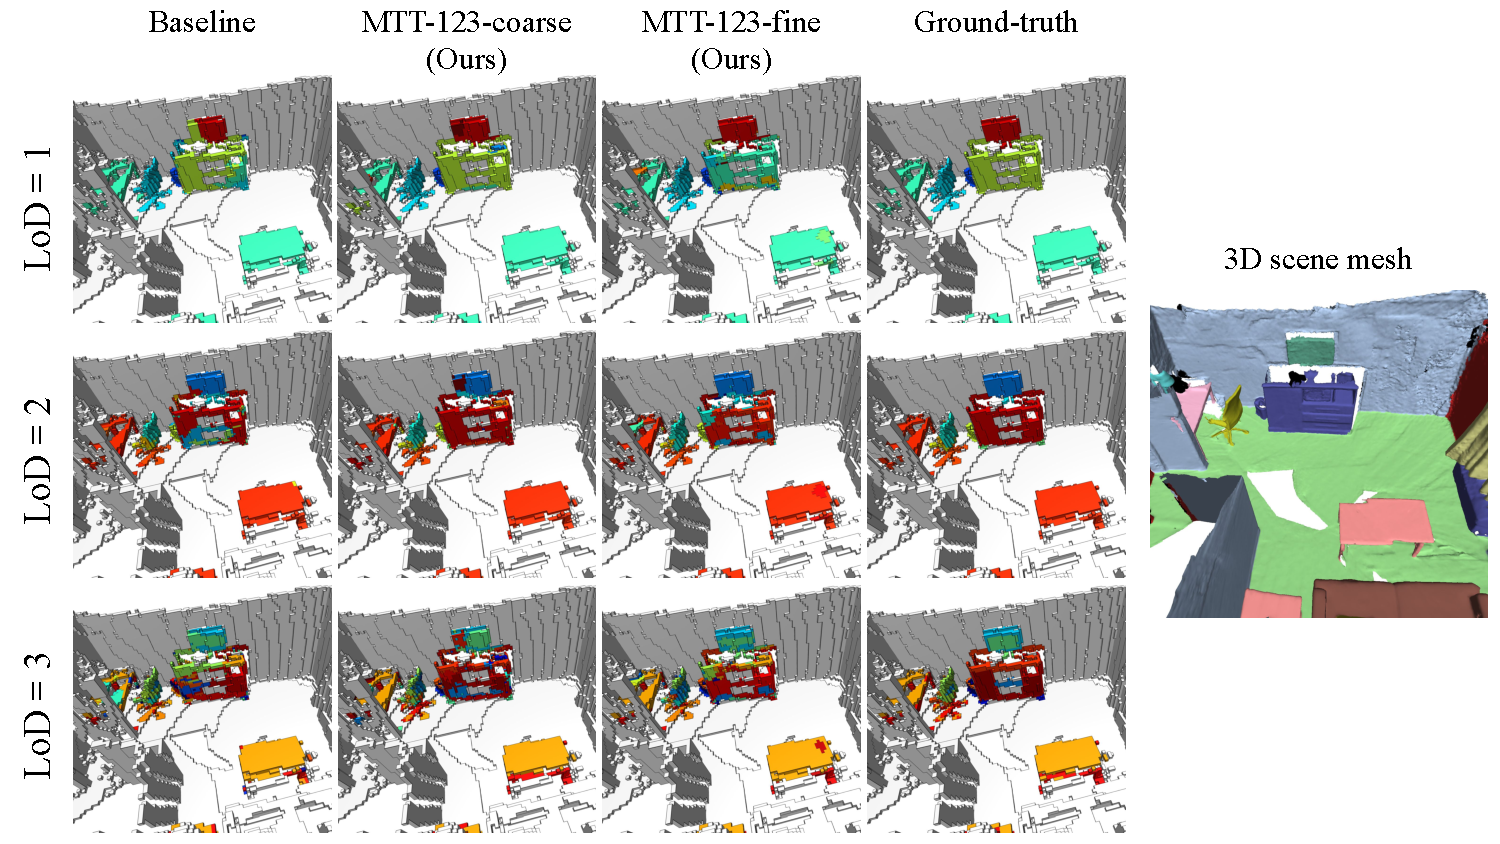
\includegraphics[width=\textwidth]{images/semantic_experiments.pdf}
\caption{Qualitative semantic labeling results}
\end{figure}

\subsection{Hierarchical semantic segmentation}
\label{supsec:results:hierarchical-segmentation}

% \AN{3 tables with class/part-wise results on hierarchical semantic segmentation for 3 different levels of detail}
\begin{table}[!htb]
\caption{results of the models on Hierarchical Segmentation task on coarse level of detail}
\begin{tabular}{lrr}
\toprule
{} &  balanced\_accuracy\_score &  iou \\
\midrule
Microwave/microwave                &                      3.0 &  1.9 \\
Bowl/bowl                          &                      0.0 &  0.0 \\
Display/display                    &                     55.0 & 38.4 \\
Faucet/faucet                      &                      0.0 &  0.0 \\
Lamp/lamp                          &                     31.3 &  9.3 \\
Laptop/laptop                      &                     11.7 &  3.0 \\
Bag/bag                            &                     29.6 &  6.7 \\
StorageFurniture/storage\_furniture &                     59.7 & 49.6 \\
Clock/clock                        &                      5.6 &  0.1 \\
Bed/bed                            &                     49.1 & 31.9 \\
Table/table                        &                     69.9 & 42.5 \\
Chair/chair                        &                     55.7 & 44.0 \\
Hat/hat                            &                      --- &  --- \\
Dishwasher/dishwasher              &                      0.0 &  0.0 \\
TrashCan/trash\_can                 &                     29.7 & 21.8 \\
Vase/pot                           &                      0.5 &  0.3 \\
Bottle/bottle                      &                      --- &  --- \\
Keyboard/keyboard                  &                     18.5 &  3.5 \\
\bottomrule
\end{tabular}
\end{table}

\begin{table}[!htb]
\caption{results of the models on Hierarchical Segmentation task on middle level of detail}
\begin{tabular}{lrr}
\toprule
{} &  balanced\_accuracy\_score &  iou \\
\midrule
Microwave/body           &                      3.2 &  2.0 \\
Bowl/container           &                      0.0 &  0.0 \\
Display/accessories      &                      --- &  0.0 \\
Faucet/normal\_faucet     &                      0.0 &  0.0 \\
Lamp/wall\_lamp           &                      0.0 &  0.0 \\
Laptop/screen\_side       &                     20.8 &  4.1 \\
Bag/luggage              &                      0.0 &  0.0 \\
StorageFurniture/cabinet &                     60.2 & 50.0 \\
Clock/normal\_clock       &                      0.0 &  0.0 \\
Bed/regular\_bed          &                     48.7 & 30.3 \\
Table/desk               &                      6.5 &  3.7 \\
Table/regular\_table      &                     71.2 & 42.5 \\
Chair/chair\_base         &                     45.9 & 37.7 \\
Hat/normal\_hat           &                      --- &  --- \\
Lamp/table\_lamp          &                     31.7 &  9.5 \\
Dishwasher/body          &                      0.0 &  0.0 \\
TrashCan/outside\_frame   &                      0.0 &  0.0 \\
Chair/chair\_arm          &                     29.4 & 12.8 \\
Bed/bunk\_bed             &                      0.8 &  0.8 \\
Chair/chair\_seat         &                     46.0 & 32.8 \\
TrashCan/container       &                     32.1 & 23.0 \\
Vase/containing\_things   &                      0.4 &  0.3 \\
Bottle/normal\_bottle     &                      --- &  --- \\
Bag/hand\_or\_shoulder\_bag &                     12.4 &  1.5 \\
Lamp/floor\_lamp          &                      0.0 &  0.0 \\
StorageFurniture/chest   &                      3.0 &  0.6 \\
Table/game\_table         &                      2.6 &  1.1 \\
Laptop/base\_side         &                      0.0 &  0.0 \\
TrashCan/cover           &                      4.4 &  2.8 \\
Chair/chair\_back         &                     40.1 & 31.5 \\
Display/base             &                     27.3 & 12.0 \\
Laptop/connector         &                      0.0 &  0.0 \\
Vase/base                &                      0.0 &  0.0 \\
Bag/paper\_bag            &                     22.2 &  5.7 \\
Keyboard/other           &                      --- &  --- \\
Lamp/street\_lamp         &                      --- &  0.0 \\
TrashCan/base            &                      0.8 &  0.4 \\
Display/display\_screen   &                     55.8 & 40.3 \\
Chair/chair\_head         &                      6.3 &  2.5 \\
Keyboard/frame           &                     11.8 &  2.6 \\
Dishwasher/base          &                      0.0 &  0.0 \\
Bag/briefcase            &                      --- &  --- \\
Bed/loft\_bed             &                     14.3 &  6.1 \\
Bowl/bottom              &                      --- &  --- \\
Keyboard/tilt\_leg        &                      0.0 &  0.0 \\
TrashCan/other           &                      0.0 &  0.0 \\
Vase/body                &                      0.8 &  0.3 \\
Microwave/base           &                      0.0 &  0.0 \\
Table/picnic\_table       &                      0.0 &  0.0 \\
Keyboard/key             &                     13.0 &  1.5 \\
\bottomrule
\end{tabular}
\end{table}

\paragraph{Qualitative hierarchical semantic segmentation results}
\label{supsec:results:hierarchical-segmentation-qualitative}

% \VI{DONE: add figure with more visualizations}
%  6. Несколько дополнительных результатов работы алгоритма (нет) (наподобие рисунка 4 основной статьи)

\begin{figure}[!t]
\label{fig:hierarchy_experiments}
\centering
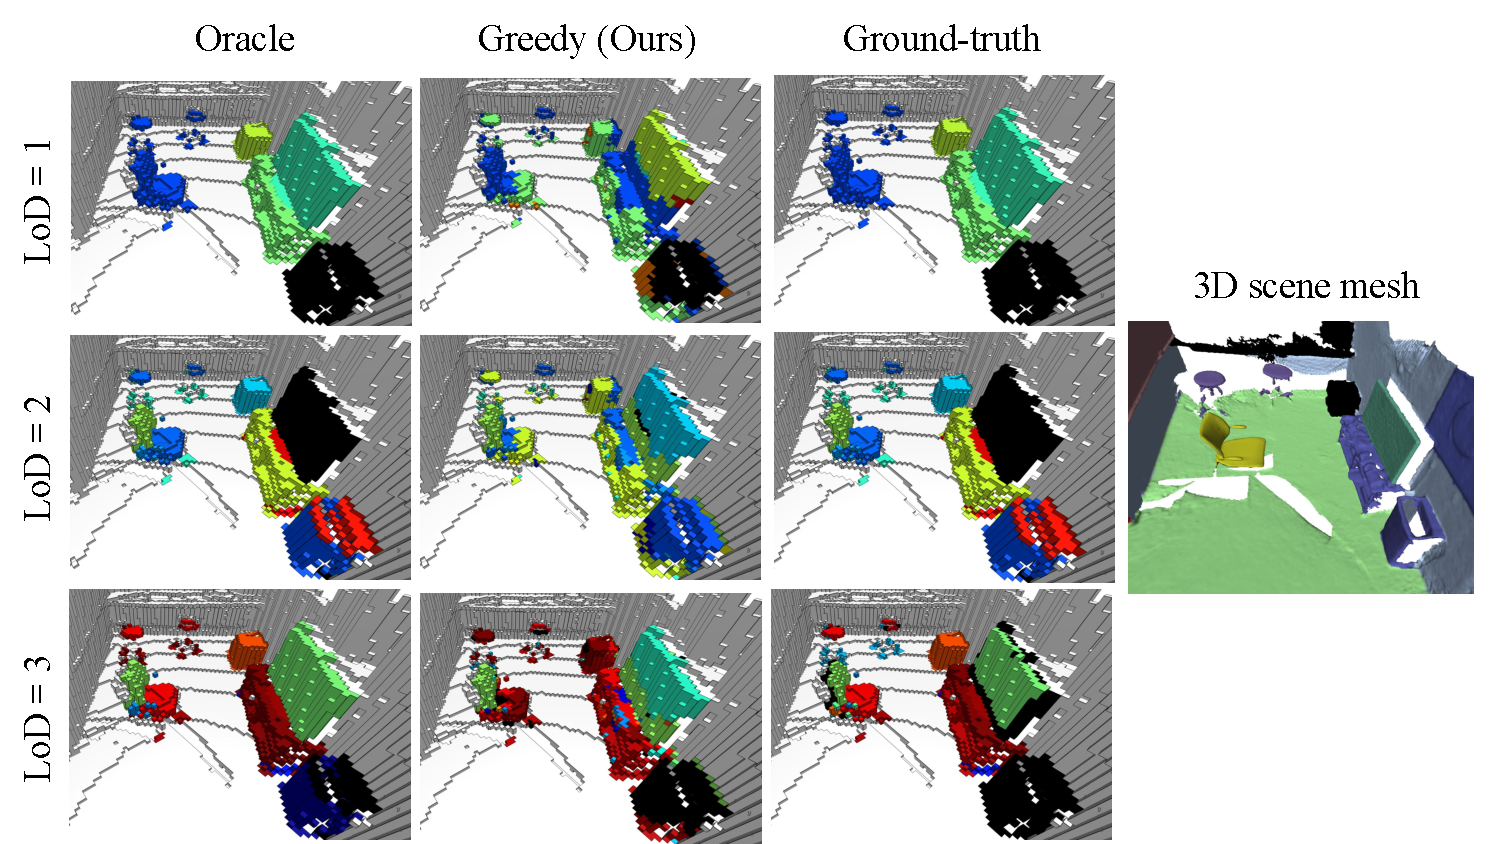
\includegraphics[width=\textwidth]{images/hierarchy_experiments.pdf}
\caption{Qualitative hierarchical semantic segmentation results}
\end{figure}


\subsection{Semantic instance segmentation}
\label{supsec:results:instance-segmentation}

% \AN{3 tables with part-wise results on semantic instance segmentation for 3 different levels of detail}

\begin{table}[!htb]
\caption{results of the models on Instance Segmentation task, original model and with background push}
% \resizebox{\textwidth}{!} & \textbf{87.50\%} & \textbf{33.33\%} & 80.59\% & 75.00\% & 28.57\% \\
Display & \textbf{76.15\%} & \textbf{64.62\%} & 29.58\% & 73.59\% & 64.00\% & \textbf{33.80\%} \\
Lamp & 65.29\% & 75.00\% & \textbf{34.62\%} & \textbf{70.64\%} & \textbf{77.78\%} & 26.92\% \\
Laptop & \textbf{50.44\%} & \textbf{100.00\%} & \textbf{9.09\%} & NaN & 0.00\% & 0.00\% \\
Bag & 89.19\% & \textbf{100.00\%} & \textbf{33.33\%} & \textbf{91.70\%} & 75.00\% & 27.27\% \\
Storage & \textbf{82.01\%} & 71.71\% & 37.30\% & 81.44\% & \textbf{74.70\%} & \textbf{38.10\%} \\
Bed & \textbf{79.55\%} & 62.86\% & 63.77\% & 78.38\% & \textbf{74.29\%} & \textbf{75.36\%} \\
Table & 77.34\% & 77.10\% & 42.49\% & \textbf{80.35\%} & \textbf{81.37\%} & \textbf{46.20\%} \\
Chair & 82.88\% & 82.14\% & 30.50\% & \textbf{86.01\%} & \textbf{86.79\%} & \textbf{32.23\%} \\
Dishwasher & 71.32\% & 100.00\% & 66.67\% & \textbf{72.66\%} & \textbf{100.00\%} & \textbf{66.67\%} \\
TrashCan & 87.22\% & \textbf{86.18\%} & \textbf{53.27\%} & \textbf{89.88\%} & 85.12\% & 51.76\% \\
Vase & \textbf{90.83\%} & 100.00\% & 33.33\% & 80.89\% & \textbf{100.00\%} & \textbf{55.56\%} \\
\hline
mIoU / mAP & 78.60\% & \textbf{83.93\%} & 35.94\% & \textbf{80.56\%} & 74.50\% & \textbf{37.11\%}
\end{tabular}%
\label{tab:lod1instsegresults}
% }
\end{table}

\begin{table}[!htb]
\caption{Instance Segmentation results on middle level of detail}
\begin{tabular}{lrrrr}
\toprule
{} &  iou &  precision &  recall &  num\_instances \\
\midrule
Microwave/body           & 74.4 &       45.5 &    23.8 &             21 \\
Laptop/screen\_side       & 99.0 &      100.0 &    50.0 &              2 \\
StorageFurniture/cabinet &  --- &        --- &     0.0 &              1 \\
Bed/regular\_bed          &  --- &        --- &     0.0 &              2 \\
Table/desk               &  --- &        0.0 &     0.0 &             11 \\
Table/regular\_table      &  --- &        --- &     0.0 &              4 \\
Chair/chair\_base         & 78.0 &       68.9 &    34.9 &            496 \\
Lamp/table\_lamp          & 76.0 &      100.0 &   100.0 &              2 \\
Dishwasher/body          & 72.3 &       49.2 &    46.4 &             69 \\
TrashCan/outside\_frame   & 52.5 &       26.7 &     3.4 &            118 \\
Chair/chair\_arm          & 76.0 &       61.7 &    32.3 &            539 \\
Bed/bunk\_bed             & 76.5 &       70.7 &    21.3 &            746 \\
TrashCan/container       & 69.8 &       75.0 &    46.2 &             26 \\
Vase/containing\_things   & 71.6 &       66.7 &    66.7 &              6 \\
Bag/hand\_or\_shoulder\_bag & 70.6 &      100.0 &    57.1 &              7 \\
Lamp/floor\_lamp          & 59.1 &       11.8 &     2.6 &            421 \\
StorageFurniture/chest   &  --- &        0.0 &     0.0 &             21 \\
Table/game\_table         & 71.9 &       67.8 &    20.9 &            748 \\
Laptop/base\_side         & 82.6 &       82.4 &    42.6 &            197 \\
TrashCan/cover           & 62.6 &       27.3 &    33.3 &              9 \\
Display/base             &  --- &        --- &     0.0 &             27 \\
Vase/base                &  --- &        --- &     0.0 &              1 \\
Bag/paper\_bag            & 87.1 &       50.0 &     2.5 &             40 \\
TrashCan/base            &  --- &        --- &     0.0 &              3 \\
Display/display\_screen   &  --- &        --- &     0.0 &              7 \\
Chair/chair\_head         & 64.1 &       50.0 &     5.4 &             37 \\
Keyboard/frame           & 73.6 &       62.4 &    17.1 &            735 \\
Dishwasher/base          &  --- &        0.0 &     0.0 &            106 \\
Bed/loft\_bed             &  --- &        --- &     0.0 &              1 \\
TrashCan/other           &  --- &        0.0 &     0.0 &              2 \\
Vase/body                & 75.1 &       61.1 &    33.3 &             33 \\
\midrule
Mean                     & 70.5 &       54.2 &    19.7 &             93 \\
\bottomrule
\end{tabular}
\end{table}




\begin{table}[!htb]
\caption{Instance Segmentation results on fine level of detail}
\begin{tabular}{lrrrr}
\toprule
{} &  iou &  precision &  recall &  num\_instances \\
\midrule
Bowl/container                 &  --- &        --- &     0.0 &              1 \\
Lamp/lamp\_unit                 & 67.3 &       50.0 &    50.0 &              2 \\
Clock/clock\_body               & 82.5 &       52.9 &    34.6 &             26 \\
Bed/bed\_unit                   & 51.2 &      100.0 &    11.1 &              9 \\
StorageFurniture/cabinet\_frame &  --- &        --- &     0.0 &              2 \\
StorageFurniture/sink          & 61.7 &       22.8 &     6.8 &            308 \\
Table/drawer\_base              & 99.5 &      100.0 &   100.0 &              2 \\
StorageFurniture/drawer        & 74.8 &       63.2 &    62.3 &             69 \\
Table/table\_base               & 69.0 &       37.5 &    17.6 &            495 \\
Chair/regular\_leg\_base         & 53.6 &       66.7 &    26.1 &             23 \\
Microwave/frame                & 55.9 &       21.7 &     8.5 &            118 \\
Chair/arm\_holistic\_frame       &  --- &        --- &     0.0 &              1 \\
StorageFurniture/countertop    & 57.6 &       26.8 &     5.9 &            188 \\
Bed/ladder                     & 66.3 &       46.1 &    21.9 &            538 \\
Chair/seat\_surface             & 70.7 &       60.3 &    18.2 &            693 \\
Chair/arm\_slant\_bar            & 67.9 &       26.7 &    19.0 &             21 \\
Chair/other                    &  --- &        --- &     0.0 &              1 \\
Chair/armrest\_hard\_surface     &  --- &        --- &     0.0 &              2 \\
Chair/star\_leg\_base            &  --- &        0.0 &     0.0 &              3 \\
Lamp/lamp\_body                 & 54.5 &        8.3 &     2.7 &             37 \\
Table/tabletop                 &  --- &        0.0 &     0.0 &             43 \\
Chair/foot\_base                &  --- &        --- &     0.0 &             14 \\
Chair/arm\_connector            & 70.7 &       58.4 &    21.9 &            744 \\
TrashCan/frame\_vertical\_bar    & 65.7 &       46.2 &     7.2 &             83 \\
Table/foosball\_table           & 50.0 &       50.0 &     7.3 &             41 \\
Vase/plant                     & 84.4 &       66.7 &    20.0 &             10 \\
Laptop/base\_frame              & 67.2 &       30.6 &     6.4 &            173 \\
Microwave/door                 & 65.3 &       55.6 &    24.0 &            229 \\
TrashCan/cover\_frame           & 59.0 &       50.0 &     9.1 &             22 \\
Display/foot\_base              &  --- &        --- &     0.0 &              3 \\
Chair/back\_frame               & 74.2 &       63.0 &    35.8 &            537 \\
Display/surface\_base           & 56.7 &       40.0 &     5.1 &             79 \\
Bag/handle                     & 70.8 &       50.0 &     5.8 &            104 \\
Display/screen                 & 58.8 &       66.7 &    50.0 &              4 \\
TrashCan/container\_handle      &  --- &        --- &     0.0 &              1 \\
StorageFurniture/cabinet\_base  &  --- &        --- &     0.0 &              2 \\
Keyboard/frame                 & 71.2 &       62.5 &    55.6 &              9 \\
Chair/seat\_frame               &  --- &        --- &     0.0 &              7 \\
\bottomrule
\end{tabular}
\end{table}


\begin{table}[!htb]
\caption{Instance Segmentation results on fine level of detail}
\begin{tabular}{lrrrr}
\toprule
{} &  iou &  precision &  recall &  num\_instances \\
\midrule

Lamp/lamp\_base                 &  --- &        --- &     0.0 &             20 \\
StorageFurniture/object        &  --- &        --- &     0.0 &              5 \\
Chair/back\_connector           &  --- &        --- &     0.0 &              5 \\
Chair/headrest                 & 75.0 &       12.5 &     2.0 &            100 \\
Microwave/side\_controls        & 69.2 &       61.5 &    18.9 &            734 \\
Display/frame                  &  --- &        --- &     0.0 &              1 \\
TrashCan/wheel\_base            & 56.0 &       16.0 &     2.7 &            295 \\
TrashCan/frame\_holistic        &  --- &        --- &     0.0 &              2 \\
Chair/back\_support             & 71.3 &       50.0 &   100.0 &              1 \\
StorageFurniture/shelf         &  --- &        --- &     0.0 &              1 \\
Bag/bag\_body                   & 75.5 &      100.0 &    50.0 &              2 \\
Laptop/screen\_frame            & 64.9 &       26.7 &     2.1 &            193 \\
TrashCan/other\_leaf            &  --- &        0.0 &     0.0 &            105 \\
Vase/container                 &  --- &        --- &     0.0 &              1 \\
Chair/arm\_sofa\_style           &  --- &        --- &     0.0 &             24 \\
Bed/furniture                  & 56.7 &       49.2 &    20.4 &            142 \\
TrashCan/cover\_lid             &  --- &        0.0 &     0.0 &              1 \\
StorageFurniture/chest\_base    &  --- &        --- &     0.0 &              6 \\
Chair/arm\_writing\_table        & 53.3 &       11.1 &     1.3 &            158 \\
Dishwasher/frame               &  --- &        --- &     0.0 &              2 \\
Dishwasher/door                &  --- &        --- &     0.0 &             11 \\
Chair/pillow                   & 57.8 &       66.7 &    18.2 &             11 \\
Bag/shoulder\_strap             &  --- &        --- &     0.0 &              1 \\
TrashCan/container\_box         &  --- &        --- &     0.0 &              3 \\
Chair/seat\_support             &  --- &        --- &     0.0 &              9 \\
Keyboard/key                   & 61.1 &        7.7 &     0.8 &            242 \\
\midrule
Mean                           & 64.7 &       41.4 &    11.8 &             64 \\
\bottomrule
\end{tabular}
\end{table}
%  6. Несколько дополнительных результатов работы алгоритма (нет) (наподобие рисунка 4 основной статьи)




\paragraph{Qualitative semantic instance segmentation results}
\label{supsec:results:instance-segmentation-qualitative}

% \VI{DONE: add figure with more visualizations}

\begin{figure}[!t]
\label{fig:instance_experiments}
\centering
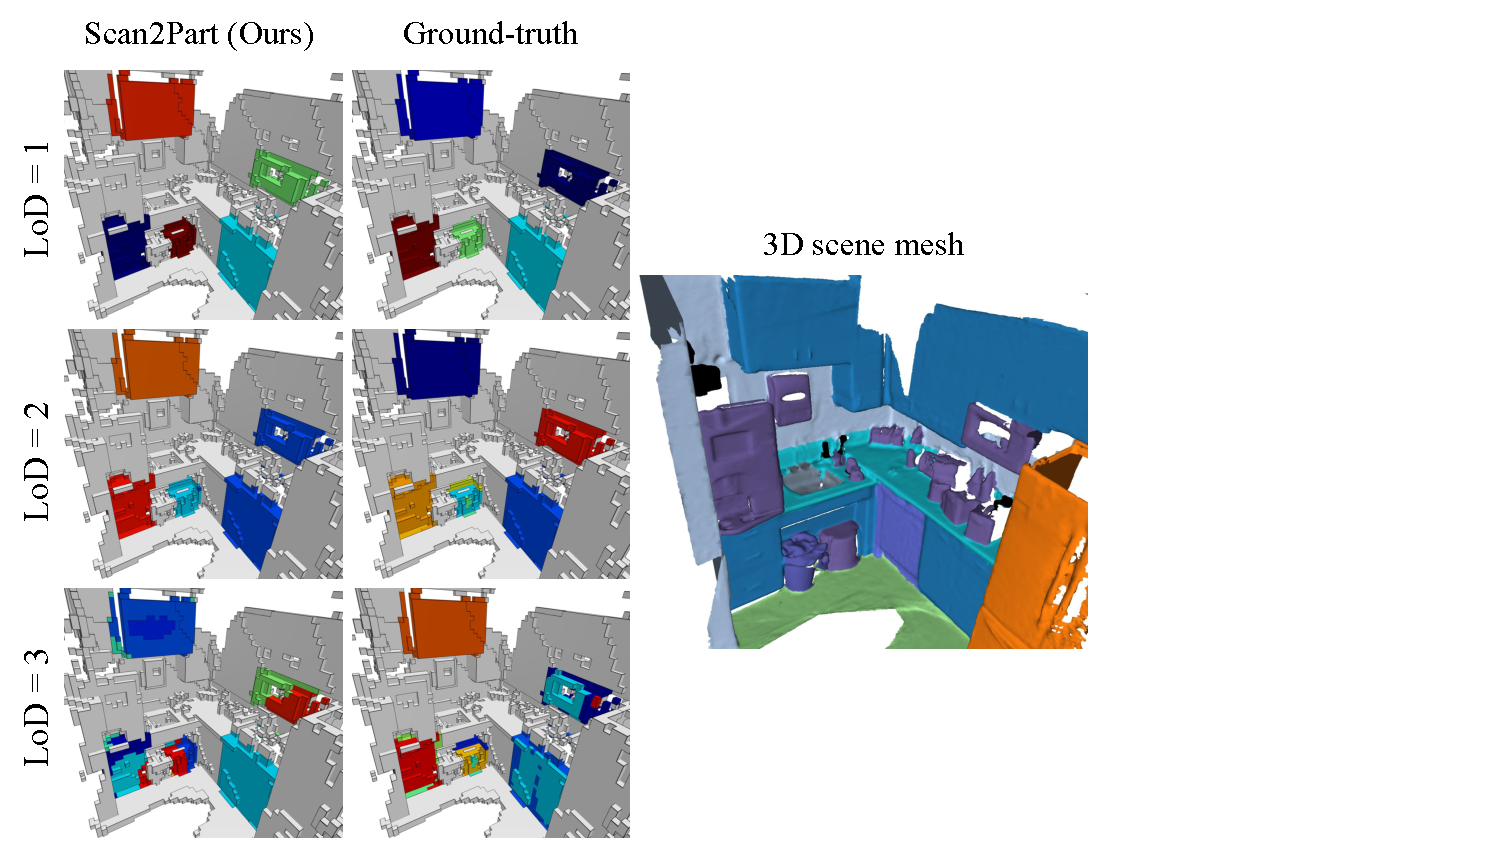
\includegraphics[width=\textwidth]{images/instance_experiments.pdf}
\caption{Qualitative semantic instance segmentation results}
\end{figure}


% % Please add the following required packages to your document preamble:
% % \usepackage{graphicx}
% {\lat
% \begin{table}[!htb]
% \caption{mIoU of different models for each class}
% \resizebox{\textwidth}{!}{%
% \begin{tabular}{l|llllll}
% Classes & Original & bg & no-w & LoD=1-2 & LoD=1-3, Dec & LoD=1-3, Inc \\
% \hline
% Microwave & 2.05\% & 0.52\% & 3.41\% & \textbf{15.86\%} & 4.74\% & 7.99\% \\
% Display & 42.28\% & 1.69\% & 41.44\% & \textbf{44.10\%} & 39.94\% & 39.01\% \\
% Lamp & 17.10\% & 0.64\% & \textbf{21.85\%} & 17.81\% & 16.47\% & 9.62\% \\
% Laptop & 9.80\% & 1.07\% & 5.60\% & 11.64\% & \textbf{11.91\%} & 6.91\% \\
% Bag & 9.97\% & 0.78\% & 4.23\% & \textbf{11.42\%} & 7.39\% & 5.98\% \\
% Storage & 47.18\% & 2.91\% & \textbf{63.40\%} & 47.10\% & 55.97\% & 44.29\% \\
% Bed & 31.98\% & 5.60\% & \textbf{53.70\%} & 46.27\% & 32.73\% & 32.78\% \\
% Table & 49.21\% & 3.96\% & \textbf{53.52\%} & 50.73\% & 46.14\% & 47.74\% \\
% Chair & 55.13\% & 3.73\% & 65.86\% & \textbf{69.67\%} & 54.07\% & 62.05\% \\
% Dishwasher & 0.00\% & 0.00\% & \textbf{8.68\%} & 0.10\% & 0.28\% & 0.00\% \\
% TrashCan & 21.35\% & 1.94\% & 28.98\% & \textbf{40.64\%} & 18.46\% & 25.80\% \\
% Vase & 1.83\% & 0.03\% & 2.00\% & \textbf{9.84\%} & 2.72\% & 1.00\% \\
% Keyboard & 4.06\% & 0.53\% & 0.26\% & 8.15\% & \textbf{11.74\%} & 1.27\% \\
% \hline
% mIoU & 22.46\% & 1.80\% & 27.15\% & \textbf{28.72\%} & 23.27\% & 21.88\%
% \end{tabular}%
% \label{tab:lodmiou1table}
% }
% \end{table}}




% \begin{figure}[!htb]
% \centering
% \label{fig:partnet_to_scannet_labeling}
% 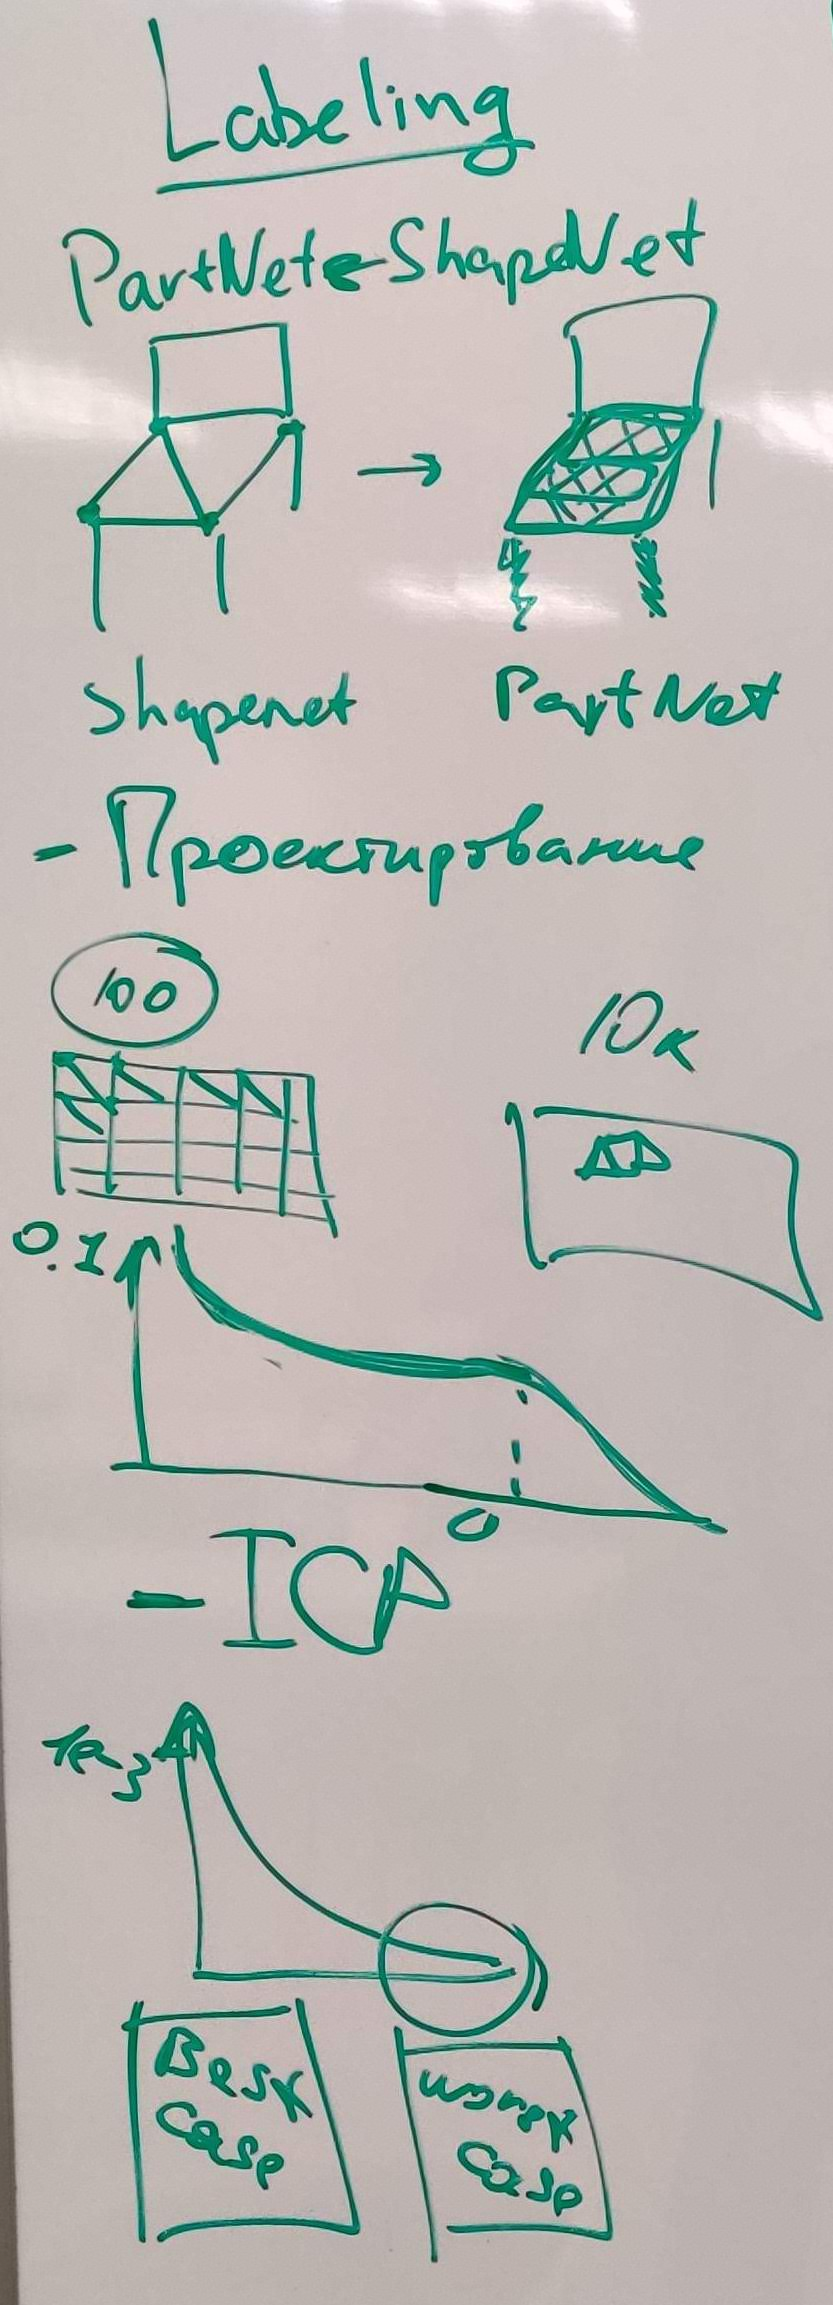
\includegraphics[trim=0 0 0 0, max width=0.25\textwidth]{images/partnet_to_scannet_labeling.jpg}
% \caption{partnet to scannet labeling (a,b,c)}
% % \end{wrapfigure}
% \end{figure}

% \begin{figure}[!htb]
% \label{fig:scannet_overview}
%   \centering
% 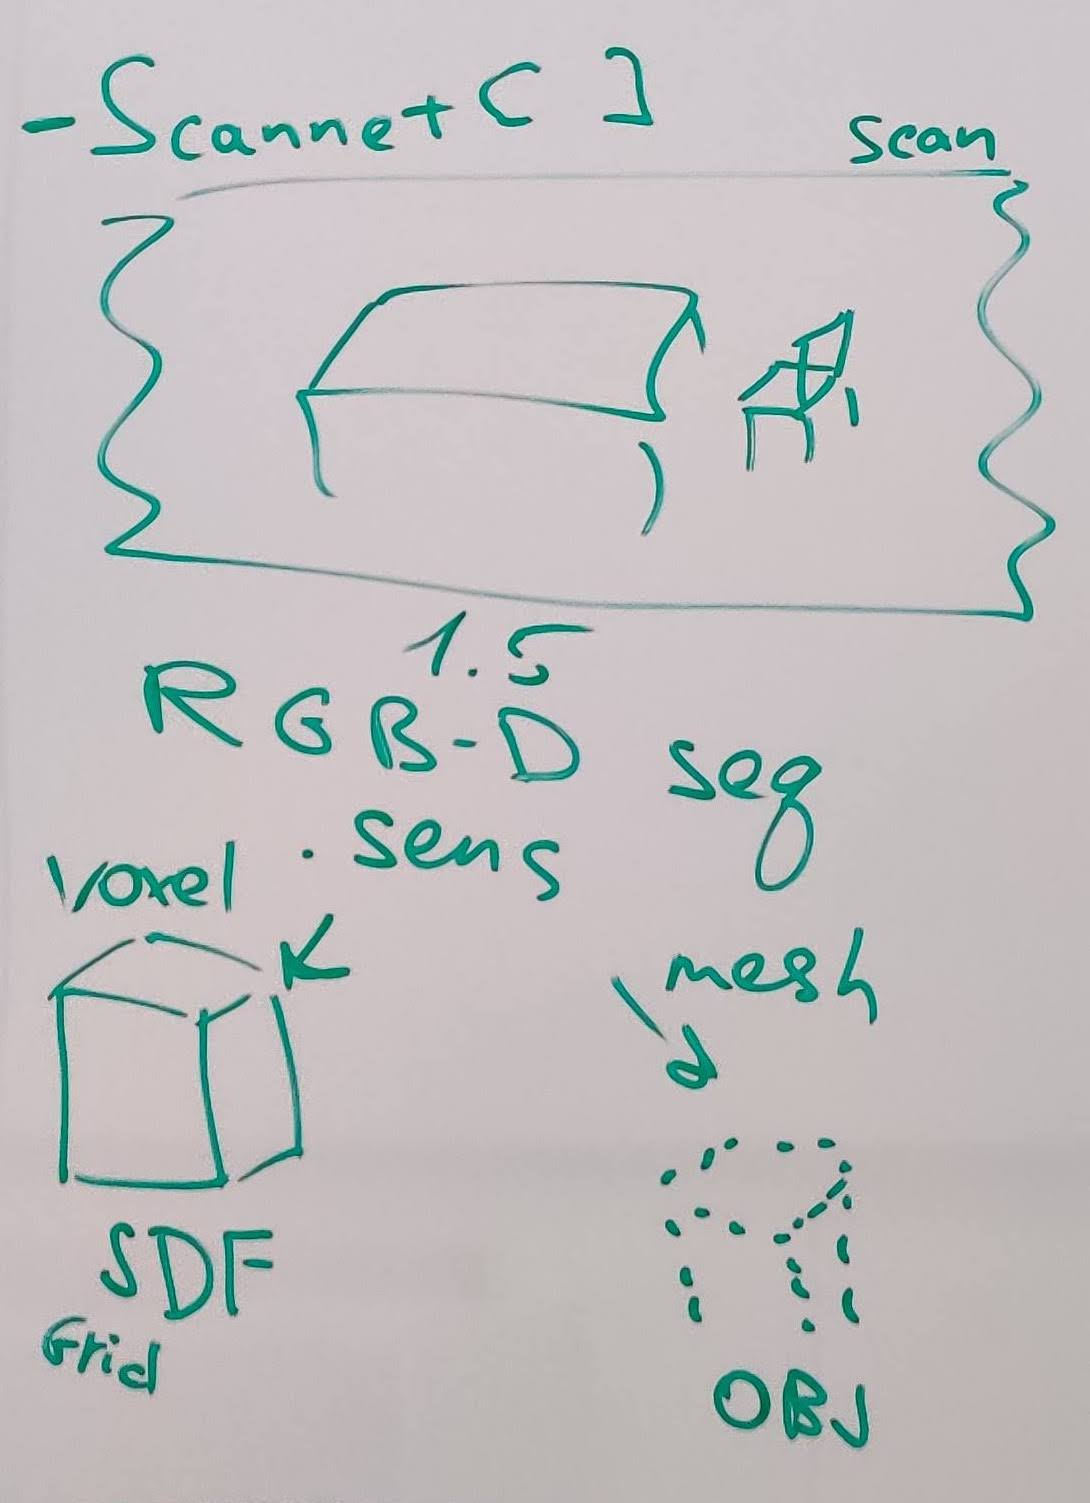
\includegraphics[trim=0 0 0 0, max width=0.5\textwidth]{images/scannet_overview.jpg}
% \caption{scannet overview}
% \end{figure}

% \begin{figure}[!htb]
% \label{fig:Scan2Cad_overview}
% \centering
% 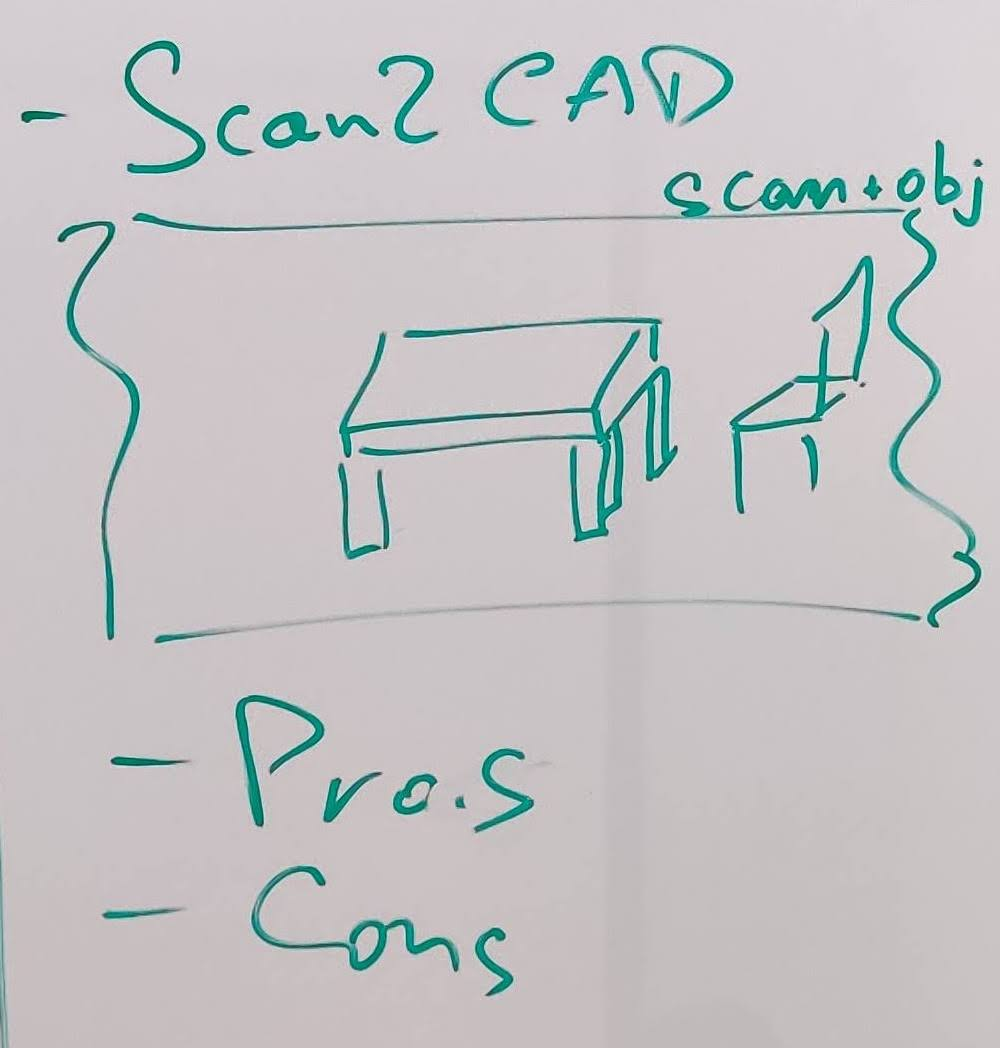
\includegraphics[trim=0 0 0 0, max width=0.5\textwidth]{images/Scan2Cad_overview.jpg}
% \caption{Scan2Cad overview}
% \end{figure}



% \begin{table}[]
% \caption{Proportions of ShapeNet semantic classes present in Scan2Cad dataset}
% \label{table:scan2part_proportions}
% \begin{tabular}{l|l|l}
% Class ID & overlap? & class name \\
% \hline
% 04379243 & 99.0\% (822/830) & table \\ \hline
% 02747177 & 98.9\% (88/89) & ashcan,trash can,garbage can,wastebin,ash bin,ash-bin \\ \hline
% 03211117 & 97.6\% (161/165) & display,video display \\ \hline
% 03761084 & 97.3\% (36/37) & microwave,microwave oven \\ \hline
% 03337140 & 97.1\% (68/70) & file,file cabinet,filing cabinet \\ \hline
% 03001627 & 96.9\% (632/652) & chair \\ \hline
% 02871439 & 96.7\% (145/150) & bookshelf \\ \hline
% 02933112 & 94.8\% (294/310) & cabinet \\ \hline
% 02818832 & 94.0\% (47/50) & bed \\ \hline
% 03991062 & 91.7\% (11/12) & pot,flowerpot \\ \hline
% 03207941 & 85.7\% (12/14) & dishwasher,dish washer,dishwashing machine \\ \hline
% 03085013 & 81.8\% (9/11) & computer keyboard,keypad \\ \hline
% 03325088 & 57.1\% (4/7) & faucet,spigot \\ \hline
% 02876657 & 50.0\% (1/2) & bottle \\ \hline
% 02808440 & 26.0\% (25/96) & bathtub,bathing tub,bath,tub \\ \hline
% 02801938 & 9.4\% (3/32) & basket,handbasket \\ \hline
% 04256520 & 8.1\% (20/247) & sofa,couch,lounge \\ \hline
% 02946921 & 0.0\% (0/1) & can,tin,tin can \\ \hline
% 03938244 & 0.0\% (0/5) & pillow \\ \hline
% 02828884 & 0.0\% (0/28) & bench \\ \hline
% 04554684 & 0.0\% (0/37) & washer,automatic washer,washing machine \\ \hline
% 03928116 & 0.0\% (0/25) & piano,pianoforte,forte-piano \\ \hline
% 03790512 & 0.0\% (0/4) & motorcycle,bike \\ \hline
% 03691459 & 0.0\% (0/2) & loudspeaker,speaker,speaker unit,loudspeaker system \\ \hline
% 03467517 & 0.0\% (0/6) & guitar \\ \hline
% 04330267 & 0.0\% (0/36) & stove \\ \hline
% 04401088 & 0.0\% (0/1) & telephone,phone,telephone set \\ \hline
% 04004475 & 0.0\% (0/31) & printer,printing machine \\ \hline
% Total:    & 81.2\% (2477/3049) &         \\
% \end{tabular}
% \end{table}




% \subsection{Scene labeling}

% \textbf{PartNet -> Shapenet.} The PartNet \cite{mo2019partnet} is a hierarchical instance-level parts dataset of labels for the subset of the ShapeNet database. The PartNet dataset is the only dataset that has a deep hierarchical structure compared to other part annotation datasets, e.g.,  \cite{Yi16}. However, the PartNet dataset does not preserve the original ShapeNet coordinate system in the sense that each object is rotated in an unspecified order. For mapping labels to Scannet scenes, we need to restore the original coordinate system. To find the rotation matrix between coordinate systems, we use the following alignment process for each object: \begin{enumerate}
%     \item we sample 20 different rotation angles corresponding to the vertices of the convex regular dodecahedron;
%     \item each rotation angle is represented as the initial alignment matrix of the object for alignment;
%     \item we perform Point-to-point ICP alignment separately for each initial alignment matrix;
%     \item we select the best one out of 20 alignment results where the distance between the original ShapeNet shape and the rotated PartNet shape is minimal.
% \end{enumerate}

% \textbf{Shapenet -> Scannet (Scan2CAD).} The Scan2CAD \cite{avetisyan2019scan2cad} is a dataset that aligns CAD objects from ShapeNet \cite{chang2015shapenet} database to scenes from Scannet. Using the marching cubes algorithm, we obtained  voxelized versions of scenes from ScanNet dataset with object type labels and mapping of coordinate systems from ScanNet to ShapeNet.  Finally, we  calculate the position of CAD object parts in the scene coordinate system and calculate relative volume in specific voxels thus projecting part labels on the scene. \DZ{unclear what relative volume is needed for here}

% Under closer examination, we discovered that most of the parts do not have a unique shape making the task of instance segmentation for parts very hard to solve and not necessary for practical scene segmentation task. \DZ{unclear}

\FloatBarrier
\clearpage

\bibliographystyle{nips}
\bibliography{references}


\end{document}
